%% (Master) Thesis template
% Template version used: v1.4
%
% Largely adapted from Adrian Nievergelt's template for the ADPS
% (lecture notes) project.


%% We use the memoir class because it offers a many easy to use features.
\documentclass[11pt,a4paper,titlepage]{memoir}

%% Packages
%% ========

%% LaTeX Font encoding -- DO NOT CHANGE
\usepackage[OT1]{fontenc}

%% Babel provides support for languages.  'english' uses British
%% English hyphenation and text snippets like "Figure" and
%% "Theorem". Use the option 'ngerman' if your document is in German.
%% Use 'american' for American English.  Note that if you change this,
%% the next LaTeX run may show spurious errors.  Simply run it again.
%% If they persist, remove the .aux file and try again.
\usepackage[english]{babel}

%% Input encoding 'utf8'. In some cases you might need 'utf8x' for
%% extra symbols. Not all editors, especially on Windows, are UTF-8
%% capable, so you may want to use 'latin1' instead.
\usepackage[utf8]{inputenc}

%% This changes default fonts for both text and math mode to use Herman Zapfs
%% excellent Palatino font.  Do not change this.
\usepackage[sc]{mathpazo}

%% The AMS-LaTeX extensions for mathematical typesetting.  Do not
%% remove.
\usepackage{amsmath,amssymb,amsfonts,mathrsfs}

%% NTheorem is a reimplementation of the AMS Theorem package. This
%% will allow us to typeset theorems like examples, proofs and
%% similar.  Do not remove.
%% NOTE: Must be loaded AFTER amsmath, or the \qed placement will
%% break
\usepackage[amsmath,thmmarks]{ntheorem}

%% LaTeX' own graphics handling
\usepackage{graphicx}

%% This allows you to add .pdf files. It is used to add the
%% declaration of originality.
\usepackage{pdfpages}

%% Some more packages that you may want to use.  Have a look at the
%% file, and consult the package docs for each.
%% See the TeXed file for more explanations

%% [OPT] Multi-rowed cells in tabulars
%\usepackage{multirow}

%% [REC] Intelligent cross reference package. This allows for nice
%% combined references that include the reference and a hint to where
%% to look for it.
\usepackage{varioref}

%% [OPT] Easily changeable quotes with \enquote{Text}
%\usepackage[german=swiss]{csquotes}

%% [REC] Format dates and time depending on locale
\usepackage{datetime}

%% [OPT] Provides a \cancel{} command to stroke through mathematics.
%\usepackage{cancel}

%% [NEED] This allows for additional typesetting tools in mathmode.
%% See its excellent documentation.
\usepackage{mathtools}

%% [ADV] Conditional commands
%\usepackage{ifthen}

%% [OPT] Manual large braces or other delimiters.
%\usepackage{bigdelim, bigstrut}

%% [REC] Alternate vector arrows. Use the command \vv{} to get scaled
%% vector arrows.
% \usepackage[h]{esvect}

%% [NEED] Some extensions to tabulars and array environments.
\usepackage{array}

%% [OPT] Postscript support via pstricks graphics package. Very
%% diverse applications.
%\usepackage{pstricks,pst-all}

%% [?] This seems to allow us to define some additional counters.
%\usepackage{etex}

%% [ADV] XY-Pic to typeset some matrix-style graphics
%\usepackage[all]{xy}

%% [OPT] This is needed to generate an index at the end of the
%% document.
%\usepackage{makeidx}

%% [OPT] Fancy package for source code listings.  The template text
%% needs it for some LaTeX snippets; remove/adapt the \lstset when you
%% remove the template content.
\usepackage{listings}
\lstset{language=TeX,basicstyle={\normalfont\ttfamily}}

%% [REC] Fancy character protrusion.  Must be loaded after all fonts.
\usepackage{microtype}

%% [REC] Nicer tables.  Read the excellent documentation.
\usepackage{booktabs}

%% Own packages
\usepackage{caption}
\usepackage{subcaption}
\captionsetup{subrefformat=parens}


%% Our layout configuration.  DO NOT CHANGE.
%% Memoir layout setup

%% NOTE: You are strongly advised not to change any of them unless you
%% know what you are doing.  These settings strongly interact in the
%% final look of the document.

% Dependencies
\usepackage{config/ETHlogo}

% Turn extra space before chapter headings off.
\setlength{\beforechapskip}{0pt}

\nonzeroparskip
\parindent=0pt
\defaultlists

% Chapter style redefinition
\makeatletter

\if@twoside
  \pagestyle{Ruled}
  \copypagestyle{chapter}{Ruled}
\else
  \pagestyle{ruled}
  \copypagestyle{chapter}{ruled}
\fi
\makeoddhead{chapter}{}{}{}
\makeevenhead{chapter}{}{}{}
\makeheadrule{chapter}{\textwidth}{0pt}
\copypagestyle{abstract}{empty}

\makechapterstyle{bianchimod}{%
  \chapterstyle{default}
  \renewcommand*{\chapnamefont}{\normalfont\Large\sffamily}
  \renewcommand*{\chapnumfont}{\normalfont\Large\sffamily}
  \renewcommand*{\printchaptername}{%
    \chapnamefont\centering\@chapapp}
  \renewcommand*{\printchapternum}{\chapnumfont {\thechapter}}
  \renewcommand*{\chaptitlefont}{\normalfont\huge\sffamily}
  \renewcommand*{\printchaptertitle}[1]{%
    \hrule\vskip\onelineskip \centering \chaptitlefont\textbf{\vphantom{gyM}##1}\par}
  \renewcommand*{\afterchaptertitle}{\vskip\onelineskip \hrule\vskip
    \afterchapskip}
  \renewcommand*{\printchapternonum}{%
    \vphantom{\chapnumfont {9}}\afterchapternum}}

% Use the newly defined style
\chapterstyle{bianchimod}

\setsecheadstyle{\Large\bfseries\sffamily}
\setsubsecheadstyle{\large\bfseries\sffamily}
\setsubsubsecheadstyle{\bfseries\sffamily}
\setparaheadstyle{\normalsize\bfseries\sffamily}
\setsubparaheadstyle{\normalsize\itshape\sffamily}
\setsubparaindent{0pt}

% Set captions to a more separated style for clearness
\captionnamefont{\sffamily\bfseries\footnotesize}
\captiontitlefont{\sffamily\footnotesize}
\setlength{\intextsep}{16pt}
\setlength{\belowcaptionskip}{1pt}

% Set section and TOC numbering depth to subsection
\setsecnumdepth{subsection}
\settocdepth{subsection}

%% Titlepage adjustments
\pretitle{\vspace{0pt plus 0.7fill}\begin{center}\HUGE\sffamily\bfseries}
\posttitle{\end{center}\par}
\preauthor{\par\begin{center}\let\and\\\Large\sffamily}
\postauthor{\end{center}}
\predate{\par\begin{center}\Large\sffamily}
\postdate{\end{center}}

\def\@advisors{}
\newcommand{\advisors}[1]{\def\@advisors{#1}}
\def\@department{}
\newcommand{\department}[1]{\def\@department{#1}}
\def\@thesistype{}
\newcommand{\thesistype}[1]{\def\@thesistype{#1}}

\renewcommand{\maketitlehooka}{\noindent\ETHlogo[2in]}

\renewcommand{\maketitlehookb}{\vspace{1in}%
  \par\begin{center}\Large\sffamily\@thesistype\end{center}}

\renewcommand{\maketitlehookd}{%
  \vfill\par
  \begin{flushright}
    \sffamily
    \@advisors\par
    \@department, ETH Z\"urich
  \end{flushright}
}

\checkandfixthelayout

\setlength{\droptitle}{-48pt}

\makeatother

% This defines how theorems should look. Best leave as is.
\theoremstyle{plain}
\setlength\theorempostskipamount{0pt}

%%% Local Variables:
%%% mode: latex
%%% TeX-master: "thesis"
%%% End:


%% Theorem environments.  You will have to adapt this for a German
%% thesis.
%% Theorem-like environments

%% This can be changed according to language. You can comment out the ones you
%% don't need.

\numberwithin{equation}{chapter}

%% German theorems
%\newtheorem{satz}{Satz}[chapter]
%\newtheorem{beispiel}[satz]{Beispiel}
%\newtheorem{bemerkung}[satz]{Bemerkung}
%\newtheorem{korrolar}[satz]{Korrolar}
%\newtheorem{definition}[satz]{Definition}
%\newtheorem{lemma}[satz]{Lemma}
%\newtheorem{proposition}[satz]{Proposition}

%% English variants
\newtheorem{theorem}{Theorem}[chapter]
\newtheorem{example}[theorem]{Example}
\newtheorem{remark}[theorem]{Remark}
\newtheorem{corollary}[theorem]{Corollary}
\newtheorem{definition}[theorem]{Definition}
\newtheorem{lemma}[theorem]{Lemma}
\newtheorem{proposition}[theorem]{Proposition}

%% Proof environment with a small square as a "qed" symbol
\theoremstyle{nonumberplain}
\theorembodyfont{\normalfont}
\theoremsymbol{\ensuremath{\square}}
\newtheorem{proof}{Proof}
%\newtheorem{beweis}{Beweis}


%% Helpful macros.
%% Special characters for number sets, e.g. real or complex numbers.
\newcommand{\C}{\mathbb{C}}
\newcommand{\K}{\mathbb{K}}
\newcommand{\N}{\mathbb{N}}
\newcommand{\Q}{\mathbb{Q}}
\newcommand{\R}{\mathbb{R}}
\newcommand{\Z}{\mathbb{Z}}
\newcommand{\X}{\mathbb{X}}

%% Fixed/scaling delimiter examples (see mathtools documentation)
\DeclarePairedDelimiter\abs{\lvert}{\rvert}
\DeclarePairedDelimiter\norm{\lVert}{\rVert}
\DeclarePairedDelimiter\bracks{\lbrack}{\rbrack}
\DeclarePairedDelimiter\ceil{\lceil}{\rceil}

%% Use the alternative epsilon per default and define the old one as \oldepsilon
\let\oldepsilon\epsilon
\renewcommand{\epsilon}{\ensuremath\varepsilon}

%% Also set the alternate phi as default.
\let\oldphi\phi
\renewcommand{\phi}{\ensuremath{\varphi}}

%% Custom commands
\newcommand{\pr}[1]{\Pr\bracks*{#1}}

\ifdefined\thesisfinal
	\newcommand{\question}[1]{}
	\newcommand{\todo}[1]{}
\else
	\newcommand{\question}[1]{\textcolor{magenta}{\textbf{Q:} #1}}
	\newcommand{\todo}[1]{\textcolor{red}{\textbf{TODO:} #1}}
\fi

\newcommand{\from}{\leftarrow}
\newcommand{\gen}{\mathrm{Gen}}
\newcommand{\enc}{\mathrm{Enc}}
\newcommand{\dec}{\mathrm{Dec}}
\newcommand{\hgen}{H_\mathrm{gen}}
\newcommand{\fhgen}{\mathcal{H}_\mathrm{gen}}
\newcommand{\qgen}{Q_\mathrm{gen}}
\newcommand{\hdep}{H_\mathrm{dep}}
\newcommand{\fhdep}{\mathcal{H}_\mathrm{dep}}
\newcommand{\qdep}{Q_\mathrm{dep}}
\newcommand{\hdh}{H_\mathrm{DH}}
\newcommand{\fdh}{F_\mathrm{DH}}
\newcommand{\fhdh}{\mathcal{H}_\mathrm{DH}}
\newcommand{\qdh}{Q_\mathrm{DH}}
\newcommand{\mdh}{m_\mathrm{DH}}
\newcommand{\qs}{Q_\mathrm{s}}
\newcommand{\ms}{m_\mathrm{s}}
\newcommand{\eeav}{\epsilon_\mathrm{EAV}}
\newcommand{\eddh}{\epsilon_\mathrm{DDH}}

% adversary
\newcommand{\adv}{\mathcal{A}}
\newcommand{\wins}{\mathcal{A} \text{ wins}}

% games and advantage
\newcommand{\game}[3]{\mathrm{Game}_{#1, #2}^{\mathrm{#3}}}
\newcommand{\advantage}[3]{\mathrm{Adv}_{#1, #2}^{\mathrm{#3}}}

% schemes
\newcommand{\dhies}{\Pi_{\mathrm{DH}}}
\newcommand{\treekem}{\Sigma_{\mathrm{TK}}}

%% ===============


%% Make document internal hyperlinks wherever possible. (TOC, references)
%% This MUST be loaded after varioref, which is loaded in 'extrapackages'
%% above.  We just load it last to be safe.
\usepackage[linkcolor=black,colorlinks=true,citecolor=black,filecolor=black]{hyperref}


%% Document information
%% ====================

\title{Tighter Security for Group Key Agreement in the Random Oracle Model}
\author{Andreas Ellison}
\thesistype{Bachelor Thesis}
\advisors{Advisors: Prof.\ Dr.\ D. Hofheinz, Dr. K. Klein}
\department{Department of Computer Science}
\date{March 16, 2024}

\begin{document}

\frontmatter

%% Title page is autogenerated from document information above.  DO
%% NOT CHANGE.
\begin{titlingpage}
	\calccentering{\unitlength}
	\begin{adjustwidth*}{\unitlength-24pt}{-\unitlength-24pt}
		\maketitle
	\end{adjustwidth*}
\end{titlingpage}

%% The abstract of your thesis.  Edit the file as needed.
\begin{abstract}
	The Messaging Layer Security (MLS) protocol, recently standardized in RFC 9420, aims to provide efficient asynchronous group key establishment with strong security guarantees. The main component of MLS, which is the source of its key efficiency and security properties, is a protocol called TreeKEM. Given that a major vision for the MLS protocol is for it to become the new standard for messaging applications like WhatsApp, Facebook Messenger, Signal, etc., it has the potential to be used by a huge number of users. Thus, it is important to better understand the security of MLS and hence also of TreeKEM. In work by Klein et.\ al, TreeKEM was proven adaptively secure in the Random Oracle Model (ROM) with a polynomial loss in security by proving a result about the security of an arbitrary IND-CPA secure public-key encryption scheme in a public-key version of the Generalized Selective Decryption (GSD) security game. \\


	In this work, we prove a tighter bound for the security of TreeKEM that implies meaningful security guarantees in practice. We follow the approach of Klein et.\ al and first introduce a modified version of the public-key GSD game better suited for analyzing TreeKEM. We then provide a simple and detailed proof of security for a specific encryption scheme, the DHIES scheme (currently the only standardized scheme in MLS), in this game in the ROM and achieve a smaller security loss compared to the result from Klein et.\ al. Finally, we state the result on the security of TreeKEM implied by this bound, and give an interpretation of the result with protocol parameters used in practice.

	\keywords{Messaging Layer Security \and TreeKEM \and Secure Messaging \and Group Key-Agreement \and Adaptive Security \and DHIES}
\end{abstract}


%% TOC with the proper setup, do not change.
\cleartorecto
\tableofcontents
\mainmatter

%% Your real content!
\chapter{Introduction}

We all rely on messaging applications like WhatsApp, Facebook Messenger, Signal, etc.\ in our daily lives and take it for granted that our messages will be transmitted securely, for some definition of ``secure''. A common security feature expected from the protocol employed in a messaging application and known also to the general public is end-to-end encryption \todo{put emphasis?}, i.e. that only the end users of a messaging session can read the messages being sent and the service provider or any party with access to the communication channel is not able to do so. Another straightforward feature is that the protocol should work in an asynchronous setting: we would like to send messages even when to recipient is offline, and we expect them to receive the messsage once they come online. For this we must rely on a server to store and deliver the messages (without being able to read them).

There are two more advanced security features expected from messaging protocols today, both related to security in case a user is compromised:
\begin{itemize}
	\item forward secrecy (FS): the compromise should not reveal the contents of old messages
	\item post-compromise security (PCS): after the user recovers from the compromise, new messages are secure once again
\end{itemize}
As a user may well not know that they have been compromised, ensuring PCS requires regularly updating the key material used for encryption (in a way that the information leaked in a compromise \emph{before} the update does not suffice to compute encryption keys used \emph{after} the update). The more often the key material can be updated, the stronger the level of PCS that is achieved. Thus, updating the key material should be an efficient operation.

For messaging between two users, the Double Ratchet protocol \cite{double-ratchet}, the main component of the so-called Signal Protocol, is a widely adopted solution used by major messaging applications such as Signal, WhatsApp, Facebook Messenger and more. It is well studied and achieves all of the above security guarantees \cite{double-ratchet-analysis}. For messaging in a group of more than two users, a straightforward solution is to maintain 1:1 communication channels using the Double Ratchet protocol between every pair of users and send messages to the group by sending them to every member individually. This achieves the same level of security as a 1:1 channel \todo{true?}, but requires a number of encryption operations linear in the group size to send a message.

Another common solution is to use ``sender keys`` \cite{sender-keys}: every user creates a symmetric key, their \emph{sender key}, and distributes this sender key to every other user using 1:1 channels as before. A user sending a message then derives a symmetric encryption key for the message from their sender key, while continually updating their sender key (with each sent message) to provide FS. However, achieving PCS is costly: if a user is compromised, the sender keys of all users are leaked and recovering from the compromise requires each user to send a new sender key to every other user over the respective 1:1 channels, resulting in a number of operations linear in the group size per user and a quadratic number of operations in total. Moreover, dynamic group membership introduces additional complexity:
\begin{itemize}
	\item adding a new member involves the new member sharing their sender key with all other group members \question{How does the new member receive the sender keys? From an existing member?}
	\item removing a member requires distributing new sender keys in the group, just like recovering from a compromise
\end{itemize}
The Messaging Layer Security (MLS) protocol, recently standardized in \cite{rfc9420}, proposes a solution for group messaging with greater efficiency and the same strong security guarantees as for the two-party case. Updating key material and adding or removing member can be achieved with a logarithmic number of operations (although the complexity may still degrade to linear in certain scenarios). At the core of MLS is a fairly recent primitive called a \emph{continuous group key agreement} (CGKA) scheme \cite{rtreekem} (this primitive was introduced only \emph{after} the first draft of the MLS protocol). In essence, a CGKA scheme enables a group of users to agree on a \emph{group key}, which they can then use to derive symmetric message encryption keys. This key must be indistinguishable from a random key for anyone outside the group eavesdropping on all communication, while also achieving FS and PCS in the face of compromises. A CGKA scheme must however also provide mechanisms for members to update their key material (enabling PCS), adding new users to the group and removing members from the group. Moreover, the scheme must work in the asynchronous setting with an untrusted server to deliver protocol messages.

The CGKA scheme used in the MLS protocol is called TreeKEM (initially proposed in \cite{treekem}) and the majority of the literature on MLS is dedicated to analyzing TreeKEM or proposing better CGKA schemes \cite{ttkem,rtreekem,insider-security,modular-group-messaging,cocoa,decaf} \todo{how many papers does it make sense to cite here? the longer the list, the more papers I haven't actually read.}. The TreeKEM protocol has undergone multiple changes since its inception. In this work we refer to the version documented in RFC 9420. TreeKEM, as adopted from its predecessors, structures a group of users as a binary tree with the group key at the root and all group members as leaves. Group members may then compute the group key, update it or add/remove other members with a number of operations logarithmic in the group size.

Given that the vision for the MLS protocol is for it to become the new standard for messaging protocols and that it has support from several large companies \cite{google-mls,mls-support}, it has the potential to be used by a huge number of users. Thus, understanding the security of MLS and hence also of TreeKEM is of great importance. This means having formal security guarantees about the security provided by TreeKEM (based on appropriate hardness assumptions). The first important step in this direction was the conception of the CGKA primitive and the accompanying definitions of security introduced in different works (for example \cite{rtreekem, ttkem}). Such definitions clarify what kind of adversaries we can provide security against and thus what kind of security one should expect from the scheme when using it in practice. Moreover, proofs of (reasonably tight) security under these definitions show what level of security we should expect from the scheme and serve as a guide to implementors on what values to choose for the security parameter. Proofs also provide strong justification that there are no flaws in the overall design of the scheme.

One choice that can be made when defining the security of a CGKA scheme is whether the adversary is modeled as \emph{selective} or \emph{adaptive}. In the former case, the adversary must provide all the interactions it will have with the protocol and when it will attempt to break the scheme at the beginning of the security game, while in the latter case the adversary can make its decisions based on responses from previous interactions. Clearly, the adaptive setting is much closer to how an attack would unfold in practice, so it is desirable to prove security against adaptive adversaries. However, achieving this without too much of a blow-up in the security loss is a challenge since one often resorts to guessing actions performed by the adversary.

The Generalized Selective Decryption (GSD) security game \cite{gsd} was introduced precisely to analyze adaptive security for protocols based on a graph-like structure (as is the case with TreeKEM). It was initially defined for the private-key setting and later adapted to the public-key setting in \cite{ttkem}. The work in \cite{ttkem} proved a polynomial bound for the adaptive security of the public-key GSD game in the so-called Random Oracle Model (ROM) for an arbitrary IND-CPA secure public-key encryption scheme. This result implies a polynomial bound for the adaptive security of TreeKEM as a CGKA as outlined also in \cite[Theorem 4]{ttkem} and subsequently proved in more detail in \cite[Theorem 12]{modular-group-messaging}.

In this work, we prove a tighter bound for the adaptive security of a more general version of the public-key GSD game in the ROM for the DHIES scheme, which is currently the only scheme specified in the MLS cipher suite. Moreover, ... .

\section{Technical overview}

\subsection{GSD}

Describe GSD

\subsection{TreeKEM}

\question{Move high level description of TreeKEM up here?}

\section{Contributions}

\todo{describe results and contribution in more detail
	\begin{itemize}
		\item own GSD definition, similar to \cite{modular-group-messaging}
		\item complete and simple proofs for GSD
		\item tighter bound
		\item clearer or improved security definitions for SD-GSD and CGKA
		\item precise statement of security loss
	\end{itemize}
}

% Following the general approach used in \cite{ttkem} to prove the security of (a variant of) TreeKEM in the ROM, we first prove a result on the GSD security of an IND-CPA secure encryption scheme in Section~\vref{sec:tighter-gsd-security}. The  We do this specifically for the DHIES scheme, which is currently the only encryption scheme specified in the MLS RFC (\cite{rfc9420}), to achieve a better reduction loss. Moreover, we will make some notable modifications to the public-key GSD game defined in \cite{ttkem}, to allow for the result to be applied to TreeKEM more directly and thus simplify the security proof.


\chapter{Preliminaries}

\section{Notation}

We will use the following notation throughout:
\begin{itemize}
	\item We write ``u.a.r.'' for ``uniformly at random''
	\item We write $x \from S$ to say that $x$ is sampled u.a.r.\ from the finite set $S$
	\item For $n \in \mathbb{N} \setminus \{0\}$, $[n] = \{1, \ldots, n\}$
	\item If $\mathbb{G}$ is a cyclic group of order $q$ and $g$ a generator, then
	      \begin{itemize}
		      \item We write the group operation in $\mathbb{G}$ multiplicatively
		      \item $h^{-1}$ denotes the inverse of $h \in \mathbb{G}$
		      \item $\log_g(h)$ denotes the unique $x \in [q]$ such that $g^x = h$
	      \end{itemize}
	\item We write $b \from \adv$ to denote the event that an adversary $\adv$ outputs the bit $b$ when playing a game where it must output a bit in the end
	\item For $a, b \in \{0, 1\}^n$, $a \oplus b$ denotes the XOR of $a$ and $b$
	\item $\log$ is short for $\log_2$
	\item We will stick to using $\kappa$ as the security parameter of private-key encryption schemes and $\eta$ as the parameter of public-key encryption schemes
	\item $\{0, 1\}^{\le l} = \bigcup_{i = 1}^{l} \{0, 1\}^i $
\end{itemize}


\section{Basic definitions}

The definitions presented in this section were taken from \cite{introduction-to-modern-cryptography}.

\subsection{Encryption schemes}

\subsubsection{Private-key encryption}

\begin{definition}[Private-key encryption {\cite[Definition 3.7]{introduction-to-modern-cryptography}}]
	Let $\kappa$ denote the security parameter. A \emph{private-key encryption scheme} $\Pi$ consists of three probabilistic polynomial-time algorithms $(\gen, \enc, \dec)$ such that:
	\begin{enumerate}[1.]
		\item The \emph{key-generation algorithm} $\gen$ takes as input $1^\kappa$ (in unary) and outputs a key $k$. We will write $k \from \gen(1^\kappa)$.
		\item The \emph{encryption algorithm} $\enc$ takes as input a key $k$ and a message $m \in \{0, 1\}^*$ , or $m \in \{0, 1\}^{\le l(\kappa)}$ for some function $l$ if the message space is finite, and outputs a ciphertext $c$. We write this as $c \from \enc_k(m)$.
		\item The deterministic \emph{decryption algorithm} $\dec$ takes as input a key $k$ and a ciphertext $c$, and outputs a message $m$ or $\bot$ (denoting an error). We write this as $m = \dec_{sk}(c)$.
	\end{enumerate}

	We may also refer to algorithm $X$ by $\Pi.X$ for $X \in \{\gen, \enc, \dec\}$.

	It is required that for every $\kappa$, every key $k$ output by $\gen$, and every message $m$, it holds that $\pr{\dec_k(\enc_k(m)) = m} = 1$ (where the probability is over the randomness of $\enc_k$).
\end{definition}

\subsubsection{Public-key encryption}

In the following definition we will be more explicit about the randomness used by the algorithm $\gen$, as we will require a way to provide the randomness as input later.

\begin{definition}[Public-key encryption {\cite[Definition 12.1]{introduction-to-modern-cryptography}}] \label{def:public-key-encryption}
	Let $\eta$ denote the security parameter.
	A \emph{public-key encryption scheme} $\Pi$ consists of three probabilistic polynomial-time algorithms $(\gen, \enc, \dec)$ such that:
	\begin{enumerate}[1.]
		\item The \emph{key-generation algorithm} $\gen$ takes as input $1^\eta$ (in unary) and outputs a pair of keys $(pk, sk)$ (a public and private key). We will write $(pk, sk) \from \gen(1^\eta)$.

		      The public key defines a message space $\mathcal{M}_{pk}$.

		      The algorithm samples up to $r(\eta)$ uniformly random bits to make randomized decisions for some function $r$ polynomial in $\eta$. The sequence of random bits $s \in \{0, 1\}^n$ with $n \ge r(\eta)$ to be used by the algorithm may also be provided as input. We write this as $(pk, sk) = \gen(1^\eta, s)$ to emphasize the fact that the output is deterministic. The algorithm must still run in time polynomial in $1^\eta$. The distribution over key pairs output by sampling $s \from \{0, 1\}^n$ and running $\gen(1^\eta, s)$ is identical to the distribution over key pairs output by running $\gen(1^\eta)$.


		\item The \emph{encryption algorithm} $\enc$ takes as input a public key $pk$ and a message $m \in \mathcal{M}_{pk}$, and outputs a ciphertext $c$. We write this as $c \from \enc_{pk}(m)$.
		\item The deterministic \emph{decryption algorithm} $\dec$ takes as input a private key $sk$ and a ciphertext $c$, and outputs a message $m$ or $\bot$ (denoting an error). We write this as $m = \dec_{sk}(c)$.
	\end{enumerate}

	We may also refer to algorithm $X$ by $\Pi.X$ for $X \in \{\gen, \enc, \dec\}$.

	It is required that for every $\eta$, every key $(pk, sk)$ output by $\gen$, and every message $m$, it holds that $\pr{\dec_{sk}(\enc_{pk}(m)) = m} = 1$ (where the probability is over the randomness of $\enc_pk$).
\end{definition}

\subsection{Security definitions}

\begin{definition}[The IND-CPA game]
	Let $\kappa$ denote the security parameter and let $\Pi$ a private-key encryption scheme. Define the game $\mathrm{Game}_{\adv, \Pi}^{\mathrm{IND-CPA}}(\kappa)$ for an adversary $\adv$:
	\begin{enumerate}[1.]
		\item A key $k \from \gen(1^\kappa)$ is generated.
		\item The adversary $\adv$ is given $1^\kappa$ and oracle access to $\Pi.\enc_k$, and outputs a pair of messages $m_0, m_1$ of the same length.
		\item A bit $b \from \{0, 1\}$ is sampled and $\adv$ is given a ciphertext $c \from \enc_k(m_b)$. ($\adv$ continues to have oracle access to $\Pi.\enc_k$.)
		\item $\adv$ outputs a bit $b'$. The output of the game is defined to be $1$ if $b' = b$, and $0$ otherwise.
	\end{enumerate}
\end{definition}

\begin{definition}[IND-CPA security {\cite[Definition 3.21]{introduction-to-modern-cryptography}}]
	A private-key encryption scheme $\Pi$ is \emph{$(t, \epsilon, q)$-IND-CPA secure} if for any adversary $\adv$ running in time $t$ we have
	\begin{align*}
		\mathrm{Adv}_{\Pi}^{\mathrm{IND-CPA}}(\adv) \coloneqq 2 \cdot \left(\pr{\mathrm{Game}_{\adv, \Pi}^{\mathrm{IND-CPA}} = 1} - \frac{1}{2}\right) \le \epsilon.
	\end{align*}
\end{definition}

We will make use of a weaker form of security called ``indistinguishability in the presence of an eavesdropper'' (\cite{introduction-to-modern-cryptography}) and will refer to it as ``EAV security''. It is identical to IND-CPA security with the sole exception that the adversary does not have access to an encryption oracle.

\begin{definition}[The EAV game]
	Let $\kappa$ denote the security parameter and $\Pi$ a private-key encryption scheme. Define the game $\mathrm{Game}_{\adv, \Pi}^{\mathrm{EAV}}$ for an adversary $\adv$:
	\begin{enumerate}[1.]
		\item A key $k \from \gen(1^\kappa)$ is generated.
		\item The adversary $\adv$ is given $1^\kappa$, and outputs a pair of messages $m_0, m_1$ of the same length.
		\item A bit $b \from \{0, 1\}$ is sampled and $\adv$ is given a ciphertext $c \from \enc_k(m_b)$.
		\item $\adv$ outputs a bit $b'$. The output of the game is defined to be $1$ if $b' = b$, and $0$ otherwise.
	\end{enumerate}
\end{definition}

\begin{definition}[EAV security {\cite[Definition 3.8]{introduction-to-modern-cryptography}}]
	A private-key encryption scheme $\Pi$ is \emph{$(t, \epsilon)$-EAV secure} if for any adversary $\adv$ running in time $t$ we have
	\begin{align*}
		\mathrm{Adv}_{\Pi}^{\mathrm{EAV}}(\adv) \coloneqq 2 \cdot \left(\pr{\mathrm{Game}_{\adv, \Pi}^{\mathrm{EAV}} = 1} - \frac{1}{2}\right) \le \epsilon.
	\end{align*}
\end{definition}


\begin{lemma}
	Let $\Pi$ a private-key encryption scheme. If $\Pi$ is $(t, \epsilon)$-IND-CPA-secure, then $\Pi$ is $(t, \epsilon)$-EAV-secure.
\end{lemma}
\begin{proof}
	This follows immediately from the fact that any EAV adversary is also an IND-CPA adversary.
\end{proof}

\begin{definition}[Group-generation algorithm {\cite[Section 9.3.2]{introduction-to-modern-cryptography}}]
	Let $\eta$ denote the security parameter. A \emph{group-generation algorithm} $\mathcal{G}$ is a deterministic polynomial-time algorithm that takes as input $1^\eta$ and outputs $(\mathbb{G}, q, g)$, where $\mathbb{G}$ is (a description of) a cyclic group, $q$ is the order of the group with $q \ge 2^\eta$ \todo{require this? probably useful for applying bound later} and $g \in \mathbb{G}$ is a generator. A group element is represented as a bit-string of length at most $\gamma(\eta)$. We write $(\mathbb{G}, q, g) \from \mathcal{G}(1^\eta)$.
\end{definition}

\begin{definition}[The Decisional Diffie-Hellman (DDH) problem]
	Let $\eta$ denote the security parameter and let $\mathcal{G}$ a group-generation algorithm.
	Define the game $\mathrm{Game}_{\adv, \mathcal{G}}^{\mathrm{DDH}}$ for an adversary $\adv$:
	\begin{enumerate}[1.]
		\item $\mathcal{G}(1^\eta)$ is run to obtain $(\mathbb{G}, q, g)$, and exponents $x, y \from [q]$ and a bit $b \from \{0, 1\}$ are sampled.
		\item The adversary $\adv$ is given $\mathbb{G}$, $q$, $g$, $h_1 \coloneqq g^x, h_2 \coloneqq g^y$ and
		      \[
			      k = \begin{cases}
				      g^{x \cdot y} & b = 0 \\
				      \tilde{k}     & b = 1
			      \end{cases}
		      \]
		      where $\tilde{k} \from \mathbb{G}$.
		\item $\adv$ outputs a bit $b'$. The output of the game is defined to be $1$ if $b' = b$, and $0$ otherwise.
	\end{enumerate}
\end{definition}

\begin{definition}[Hardness of the DDH problem {\cite[Definition 9.64]{introduction-to-modern-cryptography}}]
	The DDH problem is \emph{$(t, \epsilon)$-hard relative to} $\mathcal{G}$ if for any adversary $\adv$ running in time $t$ we have
	\begin{align*}
		\mathrm{Adv}_{\mathcal{G}}^{\mathrm{DDH}}(\adv) \coloneqq 2 \cdot \left(\pr{\mathrm{Game}_{\adv, \mathcal{G}}^{\mathrm{DDH}} = 1} - \frac{1}{2}\right) \le \epsilon.
	\end{align*}
\end{definition}

Note that by saying that ``the DDH problem is hard relative to $\mathcal{G}$'', we are simply saying that solving the Diffie-Hellman problem is hard in the (fixed) group $\mathbb{G}$ output by $\mathcal{G}(1^\eta)$. We use this phrasing as opposed to saying something along the lines of ``the DDH problem is hard in $\mathbb{G}$'', which better expresses what we mean, in order to stay closer to the formulation used in the asymptotic setting.

When analyzing the advantage of an adversary we may make use of the following well known equality.

\begin{lemma}
	Let $X$ a Bernoulli random variable and $b \from \{0, 1\}$ (where $X$ and $b$ are not necessarily independent). Then for $x \in \{0, 1\}$
	\[
		2 \cdot \left(\pr{X = b} - \frac{1}{2}\right) = \pr{X = x \mid b = x} - \pr{X = x \mid b = 1 - x}.
	\]
	In particular, if $\adv$ is an adversary with output in $\{0, 1\}$ playing a game where a bit $b \from \{0, 1\}$ is sampled, then for $x \in \{0, 1\}$
	\begin{equation} \label{eq:advantage-equality}
		2 \cdot \left(\pr{b \from \adv} - \frac{1}{2}\right) = \pr{x \from \adv \mid b = x} - \pr{x \from \adv \mid b = 1 - x}.
	\end{equation}
\end{lemma}
\begin{proof}
	Let $x \in \{0, 1\}$. We have
	\begin{align*}
		2 \cdot \left(\pr{X = b} - \frac{1}{2}\right) & = 2 \cdot \left(\pr{X = x \mid b = x} \cdot \frac{1}{2} + \pr{X = 1 - x \mid b = 1 - x} \cdot \frac{1}{2} - \frac{1}{2}\right) \\
		                                              & = \pr{X = x \mid b = x} + \pr{X = 1 - x \mid b = 1 - x} - 1                                                                    \\
		                                              & = \pr{X = x \mid b = x} - (1 - \pr{X = 1 - x \mid b = 1 - x})                                                                  \\
		                                              & = \pr{X = x \mid b = x} - \pr{X = x \mid b = 1 - x}.
	\end{align*}
\end{proof}

In the following definition we will refer to ``key-derivation functions''. This is only meant as a hint to the reader. We do not provide a definition here, as we will always model such a function as a random oracle (see Section~\vref{sec:rom}). \question{Good referenc to cite on KDFs?}

\begin{definition}[DHIES {\cite[Construction 12.19]{introduction-to-modern-cryptography}}]
	Let $\eta$ denote the security parameter. Let $\mathcal{G}$ a group-generation algorithm. Let $\Pi_s$ a private-key encryption scheme where the security parameter $\kappa$ is some function of $\eta$ and $\Pi_s.\gen(1^{\kappa(\eta)})$ samples a key u.a.r.\ from $\{0, 1\}^{\kappa(\eta)}$. Let $\mathcal{H} = \{ H_{\eta} \mid \eta \in \N \}$ a family of key-derivation functions with $H_{\eta} \colon \mathbb{G} \to \{0, 1\}^{\kappa(\eta)}$ where $\mathbb{G}$ is the group output by $\mathcal{G}(1^\eta)$. Define the algorithms $\gen, \enc$ and $\dec$ as follows:
	\begin{itemize}
		\item $\gen$: on input $1^\eta$ run $\mathcal{G}(1^\eta)$ to obtain $(\mathbb{G}, q, g)$. Sample $x \from [q]$ and set $h_1 \coloneqq g^x$. Let $H \coloneqq H_{\eta}$. Set $pk \coloneqq \langle \mathbb{G}, q, g, h_1, H \rangle$ and $sk \coloneqq \langle \mathbb{G}, q, g, x, H \rangle$, and output $(pk, sk)$.

		      The message space is the message space of $\Pi_s$ (with the security parameter set to $\kappa(\eta)$).
		\item $\enc$: on input a public key $\langle \mathbb{G}, q, g, h_1, H \rangle$ and a message $m$, sample $y \from [q]$, set $h_2 \coloneqq g^y, k \coloneqq H(h_1^y)$, compute $c' \from \Pi_s.\enc_k(m)$ and output the ciphertext $\langle h_2, c' \rangle$.
		\item $\dec$: on input a private key $\langle \mathbb{G}, q, g, x, H \rangle$ and a ciphertext $\langle h_2, c' \rangle$, compute $k \coloneqq H(h_2^x)$ and output $\Pi_s.\dec_k(c')$. If the ciphertext is not of the right form or $\Pi_s.\dec$ outputs $\bot$, output $\bot$.
	\end{itemize}
	The public-key encryption scheme $\dhies \coloneqq (\gen, \enc, \dec)$ is called the Diffie-Hellman Integrated Encryption Scheme (DHIES).

	When using the DHIES scheme later on, we will set $pk \coloneqq \langle h \rangle$ and $sk \coloneqq x$ in $\gen$, as the security parameter $\eta$ and thus $\mathbb{G}, q, g$ and $H$ are known in practice.
\end{definition}

The DHIES scheme is an instance of a so-called \emph{key-encapsulation mechanism} (\cite[Definition~12.9]{introduction-to-modern-cryptography}): a scheme that uses a public key to encapsulate a symmetric encryption key in a ciphertext and the corresponding private key to compute the encryption key again from the ciphertext. This can be combined with any arbitrary secure private-key encryption scheme to get a secure and efficient public-key encryption scheme by sending a message encrypted with the private-key encryption scheme along with an encapsulation of the encryption key.
Under the DDH assumption (i.e. the assumption that the DDH problem is hard relative to $\mathcal{G}$), using DHIES with an EAV secure private-key scheme gives an IND-CPA secure public-key encryption scheme in the ROM (see Section~\vref{sec:rom}), as proven in \cite[Theorem~12.12]{introduction-to-modern-cryptography}. Moreover, under the so-called ``gap-CDH'' assumption, also called the ``Strong Diffie-Hellman'' assumption in \cite{dhies}, using DHIES with an IND-CCA2 secure private-key encryption scheme gives an IND-CCA2 secure public-key encryption scheme (\cite[Theorem~12.22]{introduction-to-modern-cryptography}). (We do not provide defintions for many of the notions mentioned here as we will not make use of them in this work.)


\subsection{The Random Oracle Model} \label{sec:rom}

We will work in the commonly used Random Oracle Model (ROM) to prove our results. We refer the reader to \cite[Chapter 6.5]{introduction-to-modern-cryptography} for an informal overview of the ROM and to \cite{rom} for the original work that introduced the model. The ROM introduces the concept of a \emph{random oracle}. If a function $H : A \to B$ is modelled as a random oracle, then certain assumptions are made about what an adversary $\adv$ knows about $H$ and how it interacts with it:
\begin{itemize}
	\item From $\adv$'s perspective, $H$ is a black-box function. The only way for $\adv$ to interact with $H$ is for it to provide a value $a \in A$ and get back $H(a)$, and this is the only way for $\adv$ to learn $H(a)$. We say that $\adv$ \emph{queries} $H(a)$ or that $\adv$ \emph{queries $H$ for $a$}. This well-defined interface of $\adv$ to $H$ implies that a reduction can extract the queries that $\adv$ makes to $H$.
	\item From $\adv$'s perspective, $H$ is a random variable, sampled u.a.r.\ from the set of all functions from $A$ to $B$. Thus, if $\adv$ queries $H$ for some $a \in A$ that it has not queried before, the value $H(a)$ is a random variable uniformly distributed in $B$ from $\adv$'s perspective.
\end{itemize}
We do not rely on the property known as ``programmability'' in this work.


\chapter{Tighter GSD security}

\todo{Motivate GSD}

Following the general approach used in \cite{ttkem} to prove the security of (a variant of) TreeKEM in the ROM, we first prove a result on the GSD security of an IND-CPA secure encryption scheme. We do this specifically for the DHIES scheme. Moreover, we will make some notable modifications to the public-key GSD game defined in \cite{ttkem}, to allow for results to be applied to TreeKEM more directly. We motivate the modifications made later in Section~\vref{sec:application-to-treekem}.

\section{Seeded GSD with Dependencies}

We call our adaptation of GSD security \emph{Seeded GSD with Dependencies} (SD-GSD).

\todo{Explain definition in words.}
\todo{Motivate restrictions to the adversary.}
\todo{Do not allow cycles in $(V, E \cup D)$ either.}
\todo{Add remark that cycles are (maybe) ok in the ROM.}

\begin{definition}[The SD-GSD Game]

	Let $\lambda \in \N$ a security parameter. \question{Where to define $\lambda$?} Let $\Pi = (\mathrm{Gen}, \mathrm{Enc}, \mathrm{Dec})$ a public-key encryption scheme. Let $H_{\mathrm{gen}}, H_{\mathrm{dep}} \colon \{0, 1\}^\lambda \to \{0, 1\}^\lambda$ two KDFs. Define the game $\mathrm{Game}_{\adv, \Pi}^{\mathrm{SD-GSD}}$ for an adversary $\adv$:
	\begin{enumerate}[1.]
		\item \label{def:sd-gsd-game-step-1} The adversary $\adv$ outputs $n \in \N$ and a list of dependencies $D = \{(a_{i}, b_{i})\}_{i=1}^m \in [n]^2$. For each $v \in [n]$:
		      \begin{enumerate}[(i)]
			      \item \begin{itemize}
				            \item \textbf{Case $v = b_i$ for some $i$ ($v$ is the target of some dependency):} set $s_v = H_{\mathrm{dep}}(s_{a_i})$.
				            \item \textbf{Otherwise:} sample $s_v \from \{0, 1\}^\lambda$.
			            \end{itemize}
			            We call $s_v$ the \emph{seed} of the node $v$ and a tuple $(a, b) \in D$ a \emph{seed dependency}.
			      \item Compute $(sk_v, pk_v) = \gen(\hgen(s_v))$. \todo{Define what RHS means.}
		      \end{enumerate}
		      Set $\mathcal{C} = E = \varnothing$. We call the directed graph $([n], E)$ a \emph{GSD graph} of \emph{size} $n$.
		\item $\adv$ may adaptively do the following queries:
		      \begin{itemize}
			      \item $\mathrm{reveal}(v)$ for $v \in [n]$: $\adv$ is given $pk_v$.
			      \item $\mathrm{encrypt}(u, v)$ for $u, v \in [n], u \neq v$: $(u, v)$ is added to $E$ and $\adv$ is given $c \from \mathrm{Enc}_{pk_u}(s_v)$.
			      \item $\mathrm{corrupt}(v)$ for $v \in [n]$: $\adv$ is given $s_v$ and $v$ is added to $\mathcal{C}$. We call such a node $v \in \mathcal{C}$ \emph{corrupted}. All nodes not reachable from any corrupted node in the graph $([n], E \cup D)$ are \emph{safe} (while all other nodes are \emph{unsafe}) and we say their seeds are \emph{hidden} (even if an unsafe node happens to have the same seed).
		      \end{itemize}
		\item $\adv$ outputs a node $v \in [n]$. We call $v$ the \emph{challenge node}. A bit $b \from \{0, 1\}$ is sampled and $\adv$ is given
		      \[
			      r = \begin{cases}
				      \hdep(s_v) & b = 0 \\
				      s          & b = 1
			      \end{cases},
		      \]
		      where $s \from \{0, 1\}^\lambda$. $\adv$ may continue to do queries as before.
		\item \label{def:sd-gsd-game-step-4} $\adv$ outputs a bit $b'$. The output of the game is defined to be $1$ if $b' = b$, and $0$ otherwise.
	\end{enumerate}

	We require an adversary playing the above game to adhere to the following:
	\begin{itemize}
		\item The challenge node always remains a sink.
		\item The challenge node is safe.
		\item $\mathrm{reveal}$ is never queried on the challenge node.
		\item The graphs $(V, E)$ and $(V, D)$ always remain acyclic and without self-loops.
		\item All paths in the graph $(V, D)$ are vertex disjoint.
	\end{itemize}
\end{definition}

\todo{Remove random oracles from SD-GSD security and add them to Theorem~\vref{theorem:sdgsd-security} instead.}

Since we are only interested in the security of the SD-GSD game for the case where $\hgen$ and $\hdep$ are random oracles, we directly assume in our definition that the KDFs are modelled as such.

\begin{definition}[SD-GSD security in the ROM]
	A public-key encryption scheme $\Pi$ is \emph{$(t, \epsilon, N, \delta)$-SD-GSD secure} if for any adversary $\adv$ constructing a GSD graph of size at most $N$ and indegree at most $\delta$ and running in $t$ time we have
	\begin{align*}
		\mathrm{Adv}_{\Pi}^{\mathrm{SD-GSD}}(\adv) \coloneqq 2 \cdot \abs*{\pr{\mathrm{Game}_{\adv, \Pi}^{\mathrm{SD-GSD}} = 1} - \frac{1}{2}} \le \epsilon
	\end{align*}
	when $\hgen$ and $\hdep$ are random oracles.
\end{definition}

\section{Proving SD-GSD security for DHIES}

\todo{Add assumption that $\Pi_s.\gen$ samples uniformly from $\{0, 1\}^x$}
\todo{Comment on switch from IND-CPA security to EAV security.}

\begin{theorem} \label{theorem:sdgsd-security}
	Let $N, \delta \in \N$ arbitrary with $\delta \le N$. Let $\Pi_{\mathrm{DH}}$ the DHIES scheme instantiated with a private-key encryption scheme $\Pi_s$ where $\Pi_s.\gen$ samples a key uniformly at random from $\{0, 1\}^\lambda$. Let $\hdh$ the KDF and $\mathbb{G}$ the group used in $\dhies$. If $\Pi_s$ is $(t, \epsilon)$-EAV secure, the DDH problem is $(t, \epsilon)$-hard in $\mathbb{G}$ and $\hdh$ is modelled as a random oracle, then $\Pi_{\mathrm{DH}}$ is $(\tilde{t}, \tilde{\epsilon}, N, \delta)$-SD-GSD secure with
	\begin{equation*}
		\begin{split}
			\tilde{t} = t - \mathcal{O}\big(\ms + & \mdh  \\ + & N \cdot (t_{\hdep} + t_{\mathrm{sample}} + t_{\hgen} + t_{\dhies.\gen})  \\ + & N^2 \cdot t_{\dhies.\enc}\big).
		\end{split}
	\end{equation*}
	and
	\[
		\tilde{\epsilon} = \ldots
	\]
	and where $\ms$ is an upper bound on the number of queries made to either $\hgen$ or $\hdep$ and $\mdh$ is an upper bound on the number of queries made to $\mdh$. \todo{Nicer way to introduce $\ms$ and $\mdh$?}
\end{theorem}
\paragraph{Intuition}
Consider an arbitrary SD-GSD adversary $\adv$. For an execution of $\sdgsdgame{\dhies}$ we say ``\emph{$\adv$ wins}" to denote the event $\sdgsdgame{\dhies} = 1$.
As usual with random oracles we proceed by a case distinction on whether they were queried on some interesting value. Accordingly, let $Q_{\mathrm{x}}$ denote the event that $\adv$ queries $H_{\mathrm{x}}$ on a hidden seed for $x \in \{\mathrm{gen}, \mathrm{dep}\}$. (\question{What if corrupted seed is queried and it happens to coincide with a hidden seed?}) Then we can write
\begin{align*} \label{eq:theorem-sd-gsd-security-win-cases}
	\begin{split}
		\pr{\wins} & = \pr{\wins \land \qdep} + \pr{\wins \land \overline{\qdep} \,} \\
		& \stackrel{(*)}{=}  \pr{\wins \land \qdep} + \frac{1}{2}         \\
		& \le \pr{\qdep} + \frac{1}{2} \\
		& \le \pr{\qs} + \frac{1}{2},
	\end{split}
\end{align*}
where $\qs \coloneqq \qgen \cup \qdep$ ($\mathrm{s}$ for \emph{seed}).

\todo{Justify (*). (And perhaps name it better?)}

\todo{Motivate why we introduce $\qs$. (Reason: If we try to bound $\qdep$ by itself, we must separately deal with the case where the adversary was able to trigger it at a node $v$ by triggering $\qgen$ at a parent node $p$ and subsequently decrypting a ciphertext. But our argument  To eliminate this, we want to look at the point in time where either of the two events was first triggered.)}

The heart of the proof is to bound $\pr{\qs}$. When the adversary first triggers $\qs$ by querying the seed of some hidden node $w$, it can only have learned the seed through encryptions
$c_1 \from \dhies.\mathrm{Enc}_{pk_{u_1}}(s_w), \ldots, c_d \from \dhies.\mathrm{Enc}_{pk_{u_d}}(s_w)$
where $(u_1, w), \ldots, (u_d, w)$ are edges in the GSD graph (obtained through corresponding queries $\mathrm{encrypt}(u_1, w), \ldots, \mathrm{encrypt}(u_d, w)$).

\todo{Add plot illustrating edges in GSD graph and a potential seed dependency. Add note why no information is learned through $\hdh$. (No information is learned since all parent nodes of $w$ are also safe and querying $\hdh(s_p)$ for a parent $p$ would thus trigger $\qdep$.)}

The proof in \cite{ttkem} simply argued that this is not too likely if these encryptions were made with an IND-CPA secure scheme. In the context of the DHIES scheme we can say more about these encryptions and achieve a better reduction loss.
Let $x_i = \log_g(pk_{u_i})$. Each encryption $c_i$ is a tuple of the form $\langle g^{y_i}, \Pi_s.\enc_{k_i}(s_w) \rangle$ where $y_i \from [\abs{\mathbb{G}}], k_i = \hdh\left(g^{x_i \cdot y_i}\right)$. Now we can again do a case distinction on whether $\hdh$ was queried for some group element $g^{x_j \cdot y_j}$ or not.
\begin{itemize}
	\item If such a query was made, then $\adv$ solved the Diffie-Hellman challenge $(g^{x_j}, g^{y_j})$. (Remember that we assumed that $w$ is the first node for which $\qs$ is triggered and if the seed of $w$ is hidden, then so are the seeds of the nodes $u_i$. Thus the adversary has not learned the exponent $x_i$ through querying $\hgen(s_{u_i})$ for any $i$.)
	\item If no such query was made, then from $\adv$'s perspective all the $k_i$ are independent, uniformly random keys and it still was able to learn $s_w$ from the EAV secure encryptions $\Pi_s.\enc_{k_1}(s_w), \ldots, \Pi_s.\enc_{k_d}(s_w)$.
\end{itemize}
We can bound the probability of either of these events occurring using hardness of the DDH problem in $\mathbb{G}$ and EAV security of $\Pi_s$, respectively.

To this end, we call a group element $k \in \mathbb{G}$ a \emph{hidden Diffie-Hellman key} if $k = pk_u^{y_{u, w}}$, where $(u, w)$ is an edge in the GSD graph, $u$ is safe and $y_{u, w}$ is the exponent chosen in the DHIES encryption of $s_w$ (i.e. $\adv$ was given a ciphertext of the form $\langle g^{y_{u, w}}, \ldots\rangle$ when it queried $\mathrm{encrypt}(u, w)$). Now analogously to above let $\qdh$ the event that $\adv$ queries $\hdh$ on a hidden Diffie-Hellman key and let $\fdh$ the event that $\adv$ triggers $\qdh$ \emph{before} having triggered $\qs$. Then we can split of the event $\qs$ into two cases:
\begin{align*}
	\pr{\qs} & = \pr{\qs \land \fdh} + \pr{\qs \land \overline{\fdh}\,}.
\end{align*}
We bound $\pr{\qs \land \fdh}$ and $\pr{\qs \land \fdh}$ in Lemma~\ref{lemma:mi-eav-from-eav} and Lemma~\ref{lemma:eav-reduction}, respectively, which overall gives us a bound on the advantage of $\adv$ using \eqref{eq:theorem-sd-gsd-security-win-cases}.

\begin{proof}[of Theorem~\ref{theorem:sdgsd-security}]
	Let $\adv$ an arbitrary SD-GSD adversary running in time $\tilde{t}$. We will use the events defined above. We first justify step $(*)$ in \eqref{eq:theorem-sd-gsd-security-win-cases}.


	By Lemma~\vref{lemma:dh-reduction} we have
	\[
		\pr{\qs \land \fdh} \le \ldots
	\]
	and by Lemma~\vref{lemma:eav-reduction} we have
	\[
		\pr{\qs \land \overline{\fdh}\,} \le \ldots
	\]
	Then by \eqref{eq:theorem-sd-gsd-security-win-cases}
	\[
		\pr{\wins} \le x + \frac{1}{2},
	\] so
	\[
		\mathrm{Adv}_{\Pi}^{\mathrm{SD-GSD}}(\adv) \le 2 \cdot \abs*{x} = \tilde{\epsilon}.
	\]
\end{proof}

\subsection{Reducing to the DDH problem}

\begin{lemma} \label{lemma:dh-reduction}
	Let $\adv$ an SD-GSD adversary. Let $\dhies, \hdh, \mathbb{G}$ and the events $\qs, \qdh, \fdh$ as in the statement and proof of Theorem~\vref{theorem:sdgsd-security} and assume that the DDH problem is $(t, \epsilon)$-hard in $\mathbb{G}$. Then
	\[
		\pr{\qs \land \fdh} \le \ldots.
	\]
\end{lemma}
\begin{proof}
	\todo{Make a note that we only care about $\qdh$ being triggered before $\qgen$ for the proof, but we need the remaining information about $\qdep$ in Lemma~\vref{lemma:eav-reduction}}
\end{proof}

\subsection{Reducing to EAV security}

\todo{Motivation for MI-EAV}

\begin{definition}[The MI-EAV Game]
	Let $\Pi$ a private-key encryption scheme. Define the game $\mathrm{Game}_{\adv, \Pi}^{\mathrm{MI-EAV}}$ for an adversary $\adv$:
	\begin{enumerate}[1.]
		\item The adversary $\adv$ outputs $q \in \N$ and a pair of messages $m_0, m_1$ of the same length. We refer to $q$ as the number of \emph{queries} made by $\adv$.
		\item A bit $b \from \{0, 1\}$ is sampled. For each $i \in [q]$, $\adv$ is given an encryption $c_i \from \Pi.\enc_{k_i}(m_b)$ where $k_i \from \Pi.\gen()$ is generated independently from the other keys.
		\item $\adv$ outputs a bit $b'$. The output of the game is defined to be $1$ if $b' = b$, and $0$ otherwise.
	\end{enumerate}
\end{definition}

\begin{definition}[MI-EAV security]
	A private-key encryption scheme $\Pi$ is \emph{$(t, \epsilon, q)$-MI-EAV secure} if for any adversary $\adv$ making at most $q$ queries and running in time $t$ we have
	\begin{align*}
		\mathrm{Adv}_{\Pi}^{\mathrm{MI-EAV}}(\adv) \coloneqq 2 \cdot \abs*{\pr{\mathrm{Game}_{\adv, \Pi}^{\mathrm{MI-EAV}} = 1} - \frac{1}{2}} \le \epsilon.
	\end{align*}
\end{definition}

Similar to how IND-CPA security for a single encryption query implies IND-CPA security for $q$ queries with a security loss of $q$ by a standard hybrid argument, we can show that EAV security implies MI-EAV security with the same loss. Given the well known result for IND-CPA security it seems intuitive that one should be able to adapt the hybrid argument to show MI-EAV security from IND-CPA security. To see why we can make do with EAV security, recall the hybrid argument for IND-CPA security: We define the sequence of hybrid games $H_0, \ldots, H_q$ where in the game $H_i$ always the second message is encrypted for the first $i$ encryption queries and always the first for the remaining $q - i$ queries. Then given an IND-CPA adversary $\adv$ for multiple encryptions, an IND-CPA adversary $\adv'$ is constructed to bound
\[
	\abs*{\pr{\adv \text{ outputs } 1 \text{ in game } H_{i - 1}} - \pr{\adv \text{ outputs } 1 \text{ in game } H_{i}}}
\]
for arbitrary $i$.
When $\adv'$ simulates $H_{i - 1}$ or $H_{i}$ to $\adv$ depending on which message from the $i$-th query gets encrypted by the IND-CPA challenger, it makes use of the encryption oracle in the IND-CPA security game to pass on the right encryptions to $\adv$ for all other queries. Now notice that if we wanted to simulate to an MI-EAV adversary we wouldn't need access to an encryption oracle since for the MI-EAV security game all the other encryptions can easily be generated by manually sampling the new keys.

\begin{lemma} \label{lemma:mi-eav-from-eav}
	Let $\Pi$ a private-key encryption scheme with finite message space. Let $t_{\gen}, t_{\enc}$ upper bounds for the runtime of $\Pi.\gen$ and $\Pi.\enc$, respectively. If $\Pi$ is $(t, \epsilon)$-EAV secure, then for all $q \in \N$, $\Pi$ is $(\tilde{t}, q \cdot \epsilon, q)$-MI-EAV secure with $\tilde{t} = t - \mathcal{O}(q \cdot (t_\gen + t_\enc))$.
\end{lemma}
\begin{proof} Note that since the message space is finite, the time to encrypt a message is bounded. As outlined above the Lemma follows from a simple hybrid argument. Let $q \in \N$ and $\adv$ an arbitrary MI-EAV adversary running in time $\tilde{t}$ and making at most $q$ queries. Define the sequence of hybrid games $H_0, \ldots, H_q$ where in the game $H_i$ the first $i$ encryptions given to the adversary encrypt $m_1$ and all remaining encryptions encrypt $m_0$. We will write
	\[
		\pr{\adv \rightarrow 1 \mid H_i}
	\]
	for the probability of $\adv$ outputting $1$ when playing the hybrid game $H_i$.

	Let $i \in [q]$. Construct an EAV adversary $\adv'$ that behaves as follows:
	\begin{enumerate}[1.]
		\item $\adv'$ runs $\adv$ and gets $q, m_0, m_1$.
		\item $\adv'$ outputs the messages $m_0, m_1$ and gets a ciphertext $c$ from the challenger.
		\item $\adv'$ gives the ciphertexts $c_1, \ldots, c_q$ to $\adv$ where
		      \[
			      c_j = \begin{cases}
				      \Pi.\enc_{k_j}(m_1) & i < j \\
				      c                   & i = j \\
				      \Pi.\enc_{k_j}(m_0) & i > j
			      \end{cases}.
		      \]
		      and $k_j \from \Pi.\gen() \; \forall j$.
		\item $\adv'$ outputs whatever bit $\adv$ outputs.
	\end{enumerate}
	Now consider the value of the bit $b$ sampled in the EAV game. If $b = 0$, then the first $i - 1$ ciphertexts that $\adv$ received were encryptions of $m_1$ and the remaining ciphertexts were encryptions of $m_0$, where all encryptions were under keys sampled independently with $\Pi.\gen$. Thus from the view of $\adv$ everything followed the same distribution as in the game $H_{i - 1}$ and
	\[
		\pr{\adv' \rightarrow 1 \mid b = 0} = \pr{\adv \rightarrow 1 \mid H_{i - 1}}.
	\]
	Analogously, in the case $b = 1$ the first $i$ ciphertexts received by $\adv$ were encryptions of $m_1$ and the rest encryptions of $m_0$ so
	\[
		\pr{\adv' \rightarrow 1 \mid b = 1} = \pr{\adv \rightarrow 1 \mid H_{i}}.
	\]
	Then
	\begin{align} \label{eq:eav-to-mi-eav-hybrid-distinguisher}
		\begin{split}
			\begin{split}
				\abs*{\pr{\adv \rightarrow 1 \mid H_{i - 1}} - & \pr{\adv \rightarrow 1 \mid H_{i}}} \\ = {} & \abs*{\pr{\adv' \rightarrow 1 \mid b = 0} - \pr{\adv' \rightarrow 1 \mid b = 1}}
			\end{split} \\
			={} & \mathrm{Adv}_{\Pi}^{\mathrm{EAV}}(\adv')                                         \\
			\le{} & \epsilon
		\end{split}
	\end{align}
	by $(t, \epsilon)$-EAV security of $\Pi$ since $\adv'$ runs in time $\tilde{t} + \mathcal{O}(q \cdot (t_\gen + t_\enc)) = t$. Now let $b$ be the bit sampled in the MI-EAV game. Notice that
	\[
		\pr{\adv \rightarrow 1 \mid b = 0} = \pr{\adv \rightarrow 1 \mid H_0}
	\]
	and
	\[
		\pr{\adv \rightarrow 1 \mid b = 1} = \pr{\adv \rightarrow 1 \mid H_q}.
	\]
	Then
	\begin{align*}
		\mathrm{Adv}_{\Pi}^{\mathrm{MI-EAV}}(\adv) & = \abs*{\pr{\adv \rightarrow 1 \mid b = 0} - \pr{\adv \rightarrow 1 \mid b = 1}}                      \\
		                                           & = \abs*{\pr{\adv \rightarrow 1 \mid H_0} - \pr{\adv \rightarrow 1 \mid H_q}}                          \\
		                                           & = \abs*{\sum_{i = 1}^{q} \pr{\adv \rightarrow 1 \mid H_{i - 1}} - \pr{\adv \rightarrow 1 \mid H_i}}   \\
		                                           & \le \sum_{i = 1}^{q} \abs*{\pr{\adv \rightarrow 1 \mid H_{i - 1}} - \pr{\adv \rightarrow 1 \mid H_i}} \\
		                                           & \stackrel{\mathclap{\eqref{eq:eav-to-mi-eav-hybrid-distinguisher}}}{\le} q \cdot \epsilon.
	\end{align*}
\end{proof}

\begin{lemma} \label{lemma:eav-reduction}
	Let $\adv$ an SD-GSD adversary. Let $\dhies, \hdh, \ldots$ and the events $\qs, \qdh, \fdh, \ldots$ as in the statement and proof of Theorem~\vref{theorem:sdgsd-security} and assume that $\Pi_s$ is $(t, \epsilon)$-EAV secure. Then
	\[
		\pr{\qs \land \overline{\fdh}\,} \le \ldots.
	\]
\end{lemma}
\begin{proof}
	As outlined for the proof of Theorem~\vref{theorem:sdgsd-security},

	\todo{Show $\pr{\adv' \to 0 \mid b = 0} \ge \pr{\qs \land \overline{\fdh}\,}$ and $\pr{\adv' \to \mid b = 1} \le \frac{m}{2^\lambda}$.}
\end{proof}

\subsubsection{Tighter EAV security for certain schemes}

\begin{definition}[Rerandomizability]
	Let $\Pi$ a private-key encryption scheme. $\Pi$ is \emph{rerandomizable} if there exists a probabilistic algorithm $\mathrm{ReRan}$ running in time polynomial in ?, such that given $c \from \enc_k(m)$ for any $m$ and $k \from Gen()$, $\mathrm{text}$
\end{definition}

\begin{lemma}

\end{lemma}


\chapter{Application to TreeKEM} \label{sec:application-to-treekem}

\section{Continuous Group Key Agreement}

\subsection{The model}

As already described briefly in the introduction, a CGKA scheme allows a group of users to agree on a group key, indistinguishable from random for any eavesdropper, while providing mechanisms to add or remove users from the group and update the group key and users' key material, such that FS and PCS can be achieved.

Fully modelling a group of users running a CGKA scheme is complex. Since the protocol must work in the asynchronous setting, there must be a delivery service that takes protocol messages and forwards them to the recipients. Users also need to be able to publish some kind of public key, the key packages used in TreeKEM, such that they can be invited to the group with a welcome message. This functionality is also left to the delivery service. Moreover, there must be mechanisms in place to authenticate protocol messages and the published public keys.

In our model, users are honest nodes running the protocol algorithms and maintaining local state. They send out new messages and process received messages immediately. They have a reliable communication channel to the delivery service, and all public keys and protocol messages are assumed to be authenticated, meaning that an attacker cannot forge them. The delivery service, and thus an attacker, can of course see all protocol messages. We assume little about the what messages get delivered by the delivery service: the service may deliver a message to some users but not others and it may not deliver certain messages at all.

For a more complete model we refer the reader to \cite{modular-group-messaging}. The authors consider not just CGKA but the more difficult problem of \emph{secure group messaging} as tackled by the MLS protocol. The model they consider allows an attacker to inject protocol messages and gives them some control over the public keys stored by the delivery service.

\subsection{PC-CGKA schemes}

Multiple definitions of the syntax and security of CGKA schemes already exist \cite{rtreekem,ttkem,modular-group-messaging}, all meant to capture the syntax of how update, add and remove operations were performed with the latest verion of TreeKEM at the time, and all with the same name. As already described in the introduction, the current version of TreeKEM uses propose and commit operations to advance the group state, which is also the syntax formalized in \cite{modular-group-messaging} and in this work. The syntax defined in \cite{rtreekem,ttkem} came before the propose and commit syntax was introduced. In this syntax there are no proposals and every operation is a commit, either adding a single user, removing a singler group member, or just updating the key material of the committer. To differentiate our definitions from existing ones that describe something different as in \cite{rtreekem,ttkem}, we will talk about \emph{propose and commit continuous group key agreement} (PC-CGKA) schemes.

\subsubsection{Syntax}

Our definition of the syntax of PC-CGKA schemes is inspired from the definition in \cite{ttkem} and is essentially the same as what is described in \cite[Section 4.1.1]{modular-group-messaging}.

We assume that every user $u$ is identified by some value $id_u$.

\begin{definition}[PC-CGKA]
	Let $\eta$ denote the security parameter.
	A \emph{PC-CGKA scheme} $\Sigma$ with key space $\mathcal{K}$ consists of the following algorithms:
	\begin{enumerate}[1.]
		\item[] \textsc{Initialization:}
			\begin{itemize}
				\item An algorithm $\gen$. Before joining any group, a user generates a pair of keys $(pk, sk) \from \gen(1^\eta)$, a public and private key.
				\item An algorithm $\operatorname{CreateGroup}$. A user runs $\sigma \from \operatorname{CreateGroup}(1^\eta)$ to locally initialize a group with themselves as the only member and the state of the group stored in $\sigma$. We call $\sigma$ their \emph{group state}.
			\end{itemize}
		\item[] \textsc{Compute the group key:}
			\begin{itemize}
				\item An algorithm $\operatorname{Key}$. At any point in time, a member of a group with state $\sigma$ can compute the current \emph{group key} $k \from \operatorname{Key}(\sigma)$ with $k \in \mathcal{K}(\eta)$.
			\end{itemize}
		\item[] \textsc{Proposal:}
			\begin{itemize}
				\item An algorithm $\operatorname{ProposeUpdate}$. If a member $u$ of a group with state $\sigma$ wishes to update their key material, they may run $(\sigma, p) \from \operatorname{ProposeUpdate}(\sigma)$ to create an \emph{update proposal} $p$ to be shared with other members of the group and update their state such that they have processed $p$.
				\item An algorithm $\operatorname{ProposeAdd}$. If a member of a group with state $\sigma$ wishes to add a new user $u$ with public key $pk_u$ to the group, they may run $(\sigma, p) \from \operatorname{ProposeAdd}(\sigma, id_u, pk_u)$ to create an \emph{add proposal} $p$ to be shared with other members of the group and update their state such that they have processed $p$.
				\item An algorithm $\operatorname{ProposeRemove}$. If a member of a group with state $\sigma$ wishes to remove another member $u$ from the group, they may run $(\sigma, p) \from \operatorname{ProposeAdd}(\sigma, id_u)$ to create a \emph{remove proposal} $p$ to be shared with other members of the group and update their state such that they have processed $p$.
			\end{itemize}
		\item[] \textsc{Commit:}
			\begin{itemize}
				\item An algorithm $\operatorname{CreateCommit}$. To apply a list of proposals $\pi$ to the group state, a member with state $\sigma$ may run $(\sigma', c, w_{_1}, \ldots, w_{_k}) \from \operatorname{CreateCommit}(\sigma, \pi)$, where $c$ is a \emph{commit} to be shared with other members, $\sigma'$ would be the new state of the member after applying the commit\footnote{Note that the user's state is not immediately replaced with the new state output by the algorithm. We will see why in the explanation of the semantics below.} and each $w_{i}$ is a \emph{welcome message} for a newly added user.
			\end{itemize}
		\item[] \textsc{Process:}
			\begin{itemize}
				\item An algorithm $\operatorname{ProcessCommit}$. Upon receiving another member's commit $c$, a member $u$ with state $\sigma$ can set $\sigma \from \operatorname{ProcessCommit}(\sigma, c)$ to process $c$. We say that $u$ has \emph{processed} $c$.
				\item An algorithm $\operatorname{ProcessWelcome}$. Upon receving a welcome message $w$ for a user with public key $pk$, the user with this public key can set $\sigma \from \operatorname{ProcessWelcome}(pk, sk, w)$, where $sk$ is the corresponding secret key output by $\gen$.
			\end{itemize}
	\end{enumerate}

	For any object $X$ above (including $\mathcal{K}$) we will refer to it as $\Sigma.X$.

	The scheme must also specify an algorithm for determining the set of members of the group from a group state $\sigma$.
\end{definition}

\paragraph{Semantics} In the following we provide some further details regarding the semantics of the PC-CGKA algorithms:
\begin{itemize}
	\item $\gen$: The public key is used to invite the user to the group and should therefore be made public. This public key corresponds to a key package in TreeKEM (see Section~\ref{sec:treekem-overview}). The same key pair must not be reused to join multiple groups and must be discarded after it was used to join a group. A new key pair must be generated to join a new group.
	\item $\operatorname{ProposeUpdate}$: An update proposal created by a user $u$ contains (possibly public) information for the other group members about $u$'s new key material. This information is used by other members to provide encrypted information in a commit (see below) that includes the update proposal such that $u$ is able to compute the new group key.
	\item $\operatorname{CreateCommit}$: Let $c$ a commit and $w_1, \ldots, w_k$ the corresponding welcome messages output by the algorithm, run by user $u$ with group state $\sigma$ and with the proposals $\pi$ provided as input. There should be one welcome message for each new user added to the group in the commit with a corresponding add proposal in $\pi$. Welcome message $w_i$ contains the identifier $id_i$ of a user and the message should be shared with that user such that they can join the group. Besides updating the key material for all other members with an update proposal in $\pi$, the commit also updates user $u$'s key material. Accordingly, $\pi$ should not contain an update proposal for user $u$. Nor should it contain a remove proposal for user $u$ as they will know the group key resulting from the commit. User $u$ may keep both group states $\sigma$ and $\sigma'$ until the group agrees on whether to apply the commit $c$ or not. If the commit is to be applied, user $u$ sets their state to $\sigma'$ and discards $\sigma$. Otherwise, they discard $\sigma'$. Applying a commit results in a new group key.

	      Our syntax does not specify how a user learns of proposals in $\pi$ created by other users. Also how users agree on whether to apply a commit is left up to the application. The decision could be made by the delivery service or using some consensus algorithm run by all group members.

	      We see a call to $\operatorname{CreateGroup}$ as a special type of commit that is applied by the group creator.


	\item $\operatorname{ProcessCommit}$: If the commit removed the member from the group, they should not be able to compute the group key from $\sigma$ and should delete $\sigma$.
	\item $\operatorname{ProcessWelcome}$:  The user must discard their secret key $sk$ after processing a welcome message, so that the contents of the welcome message remain secret in case the user gets compromised (recall FS). As we cannot express this conveniently in our syntax, our security definition does not check for this.
\end{itemize}

\subsubsection{Correctness}

The above description of PC-CGKA schemes already provides some explicit correctness properties or implicitly implies other ones. We will explicitly define one important correctness property that a PC-CGKA scheme should satisfy in Definition~\vref{def:cgka-correctness-consistent-history}. \todo{Justify why I mention this property and why it is important. Explain examples of commit history and why it plays a role in security.}

The correctness property concerns the handling of ``bad'' (malformed or inconsistent) inputs. The algorithms of a PC-CGKA scheme should have several checks built in to deal with such inputs. For example
\begin{itemize}
	\item a commit including an update or add proposal for the commit creator is invalid
	\item a user should never process the same commit twice
	\item a user should never process a commit that they created
	\item etc.
\end{itemize}
Many of these checks are straightforward and we do not provide an extensive list of what is needed. However, we will discuss one type of check that is less straightforward and plays a role in the security of the scheme. Our correctness property enforces all members of a group to agree on the history of commits they have applied (up to joining the group). It avoids scenarios where a group member may skip a commit processed by other members that, for example, removed a user from the group. We ignore errors that would result from processing bad input in our syntax and restrict our security model to dealing with only valid inputs, as it is not our goal to analyze this type of attack on the scheme.

Before we can formally define our correctness property, we must first introduce some definitions.

\begin{definition}[Applying a commit]
	When a user
	\begin{itemize}
		\item processes commit $c$ with $\operatorname{ProcessCommit}$
		\item creates commit $c$ and subsequently updates their group state to the new state output by the corresponding call to $\operatorname{CreateCommit}$
		\item joins the group by processing welcome message $w$, where $c$ is the commit that was output along with $w$ by $\operatorname{CreateCommit}$
		\item creates a group, where we let $c$ denote the call to $\operatorname{CreateGroup}$
	\end{itemize}
	we say that the user \emph{applied} commit $c$.
\end{definition}

In the following, when talking about \emph{time} for a user that was a part of some group, we are referring to the sequence of group states they went through as members of the group\footnote{We are only interested in state transitions from applying a commit, but for completeness we will also consider transitions due to creating proposals as a part of this sequence.}.

\begin{definition}[Last commit]
	Let $u$ a user that at some point in time was a member of a group and had group state $\sigma$. We define the \emph{last commit} in $\sigma$ to be the most recent commit $c$ that $u$ applied up to arriving in state $\sigma$.
\end{definition}

In the above definition, the user's last commit will always exist since they either joined the group through a welcome message or created the group themselves.

\begin{definition}[Consistent group states] \label{def:consistent-group-state}
	Let $u_0, u_1$ two users where each user was a member of a group at some point in time. Let $\sigma_0, \sigma_1$ the group states they were in, respectively and $c_0, c_1$ the last commits in $\sigma_0, \sigma_1$, respectively. The group states $\sigma_0$ and $\sigma_1$ are said to be \emph{consistent} if $c_0 = c_1$.\footnote{If a commit is a call to $\operatorname{CreateGroup}$, it is equal to another commit iff.\ both refer to the same call to $\operatorname{CreateGroup}$. This implies that after a user just created a group, their group state is consistent with itself only.}
\end{definition}

We can now define the correctness property motivated above.

\begin{definition}[Consistent history] \label{def:cgka-correctness-consistent-history}
	A PC-CGKA scheme $\Sigma$ \emph{maintains a consistent hisory} if a user with group state $\sigma$ only successfully\footnote{As noted, we ignore checks for bad input in our syntax. To describe schemes satisfying correctness related to bad inputs, one would need to extend the syntax such that e.g.\ an algorithm can also output an error, and the user's state remains unchanged if this is the case.} processes a commit $c \from \operatorname{CreateCommit}(\sigma', \cdot)$ for some $\sigma'$\footnote{Here we only consider states $\sigma'$ that an honest user would get as output from one of the PC-CGKA algorithms.} (with $\operatorname{ProcessCommit}$) if $\sigma$ and $\sigma'$ are consistent.
\end{definition}

Definition~\ref{def:consistent-group-state} also allows us to express the following important correctness property: any set of members with consistent group states must compute the same group key with $\Sigma.\operatorname{Key}$ and must agree on the set of members of the group.

In the following we introduce a few more definitions that will become useful later.

\begin{definition}[Parent commit]
	Let $c$ a commit output by $\operatorname{CreateCommit}(\sigma_0, \cdot)$ for some $\sigma_0$. The \emph{parent commit} of $c$ is the last commit in $\sigma_0$.
\end{definition}

Note that if the PC-CGKA scheme maintains a consistent history, for a commit $c$ that was processed by a user while they were still in group state $\sigma$, the last commit in $\sigma$ will be the parent commit of $c$.

\begin{definition}[Commit history] \label{def:commit-history}
	Let $c$ a commit.\footnote{Here we only consider commits referring to a call to $\operatorname{CreateGroup}$ or output by $\operatorname{CreateCommit}$, run by an honest user.} Define the \emph{commit history} of $c$ as follows:
	\begin{itemize}
		\item \textbf{Case $c$ refers to a call to $\operatorname{CreateGroup}$:} the sequence $(c)$ of length 1
		\item \textbf{Otherwise:} the sequence $(c_1, \ldots, c_k, c)$, where $(c_1, \ldots, c_k)$ is the commit history of $c$'s parent commit $c_k$.
	\end{itemize}
\end{definition}

One could also consider the \emph{local} commit history of a group member $u$ in group state $\sigma$, consisting of the sequence of commits applied by $u$ since joining the group and until arriving in $\sigma$. If the PC-CGKA scheme maintains a consistent history, this local commit history is a suffix of the commit history of the last commit in $\sigma$. (To see this, first note that by definition the last commit in $\sigma$ is the last commit the local commit history. Then repeatedly apply the argument before Definition~\ref{def:commit-history}.) Thus, for a set of users in consistent group states, the users all agree on the commits they have processed and their order (up to the earliest commit present in the local commit history of all users).

\subsection{PC-CGKA security}

\todo{When is it okay to reset or delete key package of a user?}

Our security definition is again inspired by \cite{ttkem}. We consider fully adaptive adversaries. The adversary controls all PC-CGKA operations performed by the users, can decide who receives what messages (i.e.\ the adversary has control over the delivery service), can decide what commits get applied or discarded, and when they are discarded, by querying ``$\operatorname{confirm}$'' and can corrupt the state of any user. We will refer to commits created by a user that they have not yet been told to apply or discard as \emph{unconfirmed commits}. Corrupting a user leaks the group states corresponding to all their unconfirmed commits. Because the adversary can schedule the delivery of messages as it likes, it is possible for the adversary to create ``forks'' in the group where some users in the group are told to process one commit, while other users are told to process another. Such forks could also happen in practice and should not break security.

The adversary eventually chooses a commit to be challenged on, for which they must differentiate the group key from a uniformly random key. We must restrict the set of commits the adversary can ask to be challenged on to those that are \emph{safe} even in the face of previous or later corruptions. The level of FS and PCS expected from a PC-CGKA scheme is captured the size of this set of safe commits. Exactly which commits are considered safe will be explained later.

We also impose some notable restrictions on the adversary. The adversary cannot inject protocol messages or public keys and it may only deliver a message to users that are supposed to process that message, in order to avoid giving users messages with bad inputs. The latter restriction is justified, as in a correct PC-CGKA protocol such messages would simply be discarded and correctness can be verified independently. Imposing the restriction on the adversary allows us to ignore the details of handling bad inputs when specifying a PC-CGKA scheme and analyzing the core aspects of its security.

The definition in \cite[Section B.1]{modular-group-messaging} is very similar in essence. The same restricions on the adversary are imposed. However, the security game provided there gives more power to the adversary: the adversary may additionally choose the randomness used in operations, choose its own public keys to be associated with users and tell certain users not to delete old keys. In the end this restricts the set of safe commits. We provide our own definition with the hope of having a formulation that is easier to digest, keeps the security game simpler and is more explicit about what commits are considered safe.

\begin{definition}[The PC-CGKA game]
	Let $\eta$ denote the security parameter and let $\Sigma$ a PC-CGKA scheme. Define the game $\game{\Sigma}{\eta}{CGKA}(\adv)$ for an adversary $\adv$:
	\begin{enumerate}[1.]
		\item \label{def:cgka-game-step-init} $\adv$ outputs $n \in \mathbb{N}$. For each $i \in [n]$, initialize a user $i$ by creating a (unique) identifier $id_i$, generating $(pk_i, sk_i) \from \Sigma.\gen(1^\eta)$, preparing $U_i = \varnothing$, the set of unconfirmed commits at user $i$, and setting $\sigma_i \coloneqq \varnothing$, where $\varnothing$ denotes the empty value. The state output by an algorithm of $\Sigma$ is never the empty value. $\adv$ is given $(pk_1, id_1), \ldots, (pk_n, id_n)$.

		      Set $P = C = W = 0$, where $P$ denotes the number of proposals, $C$ the number of commits and $W$ the number of welcome messages created.
		\item $\adv$ may adaptively do the following queries:
		      \begin{itemize}
			      \item $\operatorname{create-group}(i)$ for $i \in [n]$: set $\sigma_i \from \operatorname{CreateGroup}(1^\eta)$.
			      \item $\operatorname{propose-update}(i)$ for $i \in [n], \sigma_i \neq \varnothing$: run $(\sigma_i, p_{P + 1}) \from \operatorname{ProposeUpdate}(\sigma_i)$ to update user $i$'s state and get a proposal $p_{P + 1}$. $\adv$ is given $p_{P + 1}$. Set $P \coloneqq P + 1$.
			      \item $\operatorname{propose-add}(i, j)$ for $i, j \in [n], \sigma_i \neq \varnothing$: run $(\sigma_i, p_{P + 1}) \from \operatorname{ProposeAdd}(\sigma_i, id_j, pk_j)$ to update user $i$'s state and get a proposal $p_{P + 1}$. $\adv$ is given $p_{P + 1}$. Set $P \coloneqq P + 1$.
			      \item $\operatorname{propose-remove}(i, j)$ for $i, j \in [n], \sigma_i \neq \varnothing$: run $(\sigma_i, p_{P + 1}) \from \operatorname{ProposeRemove}(\sigma_i, id_j)$ to update user $i$'s state and get a proposal $p_{P + 1}$. $\adv$ is given $p_{P + 1}$. Set $P \coloneqq P + 1$.
			      \item $\operatorname{create-commit}(i, (j_1, \ldots, j_d))$ for $i \in [n], \sigma_i \neq \varnothing, \forall l \; j_l \in [P]$: run $(\sigma, c_{C + 1}, w_{W + 1}, \ldots, w_{W + k}) \from \operatorname{CreateCommit}(\sigma_i, (p_{j_1}, \ldots, p_{j_d}))$ to create the new state $\sigma$, commit $c_{C + 1}$ and corresponding welcome messages. $\adv$ is given $c_{C + 1}$ and $w_{W + 1}, \ldots, w_{W + k}$. Set $U_i \coloneqq U_i \cup \{(C + 1, \sigma)\}$, $C \coloneqq C + 1$ and $W \coloneqq W + k$.
			      \item $\operatorname{confirm}(j, b)$ for $j$ s.t.~$(j, \sigma) \in U_i$ for some user $i$ and state $\sigma$, $b \in \{0, 1\}$: If $b = 0$, set $U_i \coloneqq U_i \setminus \{(j, \sigma)\}$. If $b = 1$, set $\sigma_i \coloneqq \sigma$ and $U_i \coloneqq \varnothing$.\footnote{All other unconfirmed commits in $U_i$ are cleared if $b = 1$ as they should not be applied anymore.}
			      \item $\operatorname{deliver-commit}(i, j)$ for $i \in [n], \sigma_i \neq \varnothing, j \in [C]$: run $\sigma \from \operatorname{ProcessCommit}(\sigma_i, c_j)$. Set $U_i \coloneqq \varnothing$. If $c_j$ contains a remove proposal for user $i$, then set $\sigma_i \coloneqq \varnothing$, generate a new pair $(pk_i, sk_i) \from \Sigma.\gen(1^\eta)$ and give $(i, pk_i)$ to $\adv$. Otherwise, set $\sigma_i \coloneqq \sigma$.
			      \item $\operatorname{deliver-welcome}(i, j)$ for $i \in [n], \sigma_i = \varnothing, j \in [W]$: set $\sigma_i \from \operatorname{ProcessWelcome}(pk_j, sk_j, w_j)$.\footnote{Note that in a real execution of the protocol the user must delete $sk_j$ from their local state after processing the welcome message $w_j$. Accordingly, $sk_j$ is no longer leaked to the adversary in a later query $\operatorname{corrupt}(j)$.}
			      \item $\operatorname{corrupt}(i)$ for $i \in [n]$: If $\sigma_i = \varnothing$, $\adv$ is given $sk_i$. Otherwise, $\adv$ is given $\sigma_i$ and $U_i$.
		      \end{itemize}
		\item $\adv$ picks $i \in [0, C]$. We call the commit $c_i$ the \emph{challenge commit}, where the $c_0$ refers to the initial $\operatorname{CreateGroup}$ operation. Let $\sigma$ the group state output by the operation that created $c_i$ (the state output by $\operatorname{CreateCommit}$ if $i > 0$ or the state output by $\operatorname{CreateGroup}$ if $i = 0$). A bit $b \from \{0, 1\}$ is sampled and $\adv$ is given
		      \[
			      k = \begin{cases}
				      \Sigma.\operatorname{Key}(\sigma) & b = 0 \\
				      \tilde{k}                         & b = 1
			      \end{cases},
		      \]
		      where $\tilde{k} \from \Sigma.\mathcal{K}(\eta)$. $\adv$ may continue to do queries as before.
		\item $\adv$ outputs a bit $b'$. The output of the game is defined to be $1$ if $b' = b$, and $0$ otherwise.
	\end{enumerate}

	We require an adversary playing the above game to adhere to the following:
	\begin{itemize}
		\item $\operatorname{create-group}$ is queried exactly once
		\item The challenge commit is safe (see Definition~\vref{def:safe-commit})
		\item For any query $\operatorname{deliver-commit}(i, j)$ where the commit $c_j$ was created by user $k$ while they where in state $\sigma_k'$, $\sigma_i$ and $\sigma_k'$ must be consistent
		\item For any query $\operatorname{create-commit}(i, (j_1, \ldots, j_d))$, for every proposal $p_{j_l}$ created by a user while in state $\sigma_l'$, $\sigma_i$ and $\sigma_l'$ must be consistent
		\item A user never processes a commit that they created
		\item Every commit is processed at most once by any user
		\item A welcome message for user $i$ is processed by $i$ at most once and is never processed by a user $j$ with $i \neq j$
		\item A user creating a commit never includes an update or remove proposal for themselves, or multiple update/add/remove proposals for to the same user
		\item A user is never asked to create an add proposal for a user they consider to be in the group, or create a remove proposal for a user they do not consider to be in the group
	\end{itemize}
	\todo{Justify the restrictions to the adversary.}
\end{definition}

The concept of a safe user and safe commit is adapted from the so-called ``safe predicate'' in \cite{ttkem}, which again took inspiration from \cite{rtreekem}. As elaborated in the cited papers and also analogous to how we needed to define ``safe'' nodes in the SD-GSD game, we want to forbid the adversary to ask to be challenged on a commit for which it can trivially compute the group key through some corruption it performed.

To see what is needed for a commit to be safe, consider some commit $c$ with group key $k$ created by a user $i$ and let $j \neq i$ any user that $i$ would consider to be in the group after applying $c$ (Definition~\ref{def:group-members-after-applying-commit} clarifies exactly which users are considered to be in the group). The commit $c$ or an associated welcome message provides encrypted information for user $j$ to compute the new group key using its current key material. Clearly, if this key material has been compromised by the adversary corrupting user $j$, the commit should not be safe. If the adversary has not corrupted user $j$ since they last updated their key material, then we would not expect the adversary to be able to learn the group key $k$ through user $j$, even if user $j$ was corrupted before (recall PCS).
Moreover, corrupting user $j$ after they have again updated their key material should not allow the adversary to compute the group key of $c$ either (recall FS). We will later say that the commit $c$ is \emph{safe with respect to user $j$} if $j$ was not corrupted in this window between their last and next update.
Now, it is important to notice that the encrypted information in commit $c$ is for the key material that user $j$ had \emph{from user $i$'s view} when user $i$ created $c$. It is possible that when user $i$ created $c$, user $j$ had already processed a commit updating their key material that user $i$ has not yet processed. Thus, we must be careful to require exactly the right key material of user $j$ to be unknown to the adversary. Definition~\vref{def:safe-commit-wrt-user} formalizes this.

\begin{definition} \label{def:group-members-after-applying-commit}
	Let $c$ a commit and let $\sigma'$ the new group state ouptut by
	\begin{itemize}
		\item the call to $\operatorname{CreateCommit}$ that created $c$
		\item or the call to $\operatorname{CreateGroup}$ that $c$ refers to
	\end{itemize}
	The (set of) \emph{users in the group after applying $c$} is the set of users in the group according to state $\sigma'$.
\end{definition}


\begin{definition} \label{def:last-update-before-commit}
	Let $c$ a commit and let $u$ a user in the group after applying $c$. Let $h = (c_1, \ldots, c_k)$ the commit history of $c$. Define $u$'s \emph{last update up to} $c$ as the last commit $c_i$ to satisfy the following:
	\begin{enumerate}[(i)]
		\item $c_i$ was created by $u$
		\item $c_i$ included an update proposal for $u$
		\item $c_i$ was output along with a welcome message for $u$
		\item $c_i$ refers to a call to $\operatorname{CreateGroup}$ run by $u$ (implying $i = 1$)
	\end{enumerate}
\end{definition}

\begin{definition}[Safe user] \label{def:safe-commit-wrt-user}
	Let $\eta$ arbitrary and let $\Sigma$ a PC-CGKA scheme. Consider an execution of $\game{\Sigma}{\eta}{CGKA}(\adv)$ for some adversary $\adv$. Let $Q$ the total number of queries made by $\adv$. We will refer to queries by their index among all queries. Let $q^* \in [Q]$ a $\operatorname{create-group}(i)$ or $\operatorname{create-commit}(i, \cdot)$ query with $i \in [n]$ as the target user. Let $j \in [n]$ any user (including $i$) in the group after applying the commit $c^*$ created by $q^*$. Let the commit $c'$ be user $j$'s last update up to $c^*$.

	Set the query $q^- \in [Q]$ depending on which case in Definition~\ref{def:last-update-before-commit} commit $c'$ falls into:
	\begin{enumerate}[(i)]
		\item $q^-$ is the $\operatorname{create-commit}(j, \cdot)$ query that created $c'$
		\item $q^-$ is the $\operatorname{propose-update}(j)$ query that created the update proposal for $j$ included in $c'$
		\item $q^-$ is the last $\operatorname{deliver-commit}$ query before $q^*$ that reset $j$'s public and private key pair or $q^- = 0$ if no such query was made
		\item $q^-$ is the corresponding query $\operatorname{create-group}(j)$ that ran $\operatorname{CreateGroup}$
	\end{enumerate}

	\todo{Simplify this case if possible.}

	Again, set the query $q^+ \in [Q]$ depending on which case in Definition~\ref{def:last-update-before-commit} commit $c'$ falls into:
	\begin{enumerate}[(i)]
		\item \begin{itemize}
			      \item \textbf{Case user $j$ applied $c'$, i.e. a query $\operatorname{confirm}(k, 1)$ with index $q_{\mathrm{confirm}}$ was made where $c_k = c'$:} same as $(iv)$, but use the next query after $q_{\mathrm{confirm}}$.
			      \item \textbf{Otherwise:} $q^+$ is the next query that removed the new state associated with $c'$ from $U_j$. This is either a query $\operatorname{confirm}(k, 0)$ with $c_k = c'$, a query $\operatorname{confirm}(k, 1)$ with $c_k \neq c'$ or a query $\operatorname{deliver-commit}(j, k)$ with $c_k \neq c'$. Set $q^+ = Q$ if there is no such query.
		      \end{itemize}
		\item Let $p$ be the update proposal for $j$ included in $c'$.
		      \begin{itemize}
			      \item \textbf{Case $j$ applied a commit $c_k$ that included $p$}: same as $(iv)$, but use the next query after $q_{\mathrm{deliver}}$, where $q_{\mathrm{deliver}}$ is the $\operatorname{deliver-commit}(j, k)$ query that let $j$ process $c_k$
			      \item \textbf{Otherwise:} $q^+$ is the next query $q > q^-$ that led to user $j$ applying a commit $c$ that included a remove proposal for $j$, or set $q^+ = Q$ if no such commit exists \todo{explain this: the user will keep the new key material associated with the update proposal around in its state, so the key material is only deleted when $j$ is removed from the group}
		      \end{itemize}
		\item same as $(iv)$ \todo{Note: here we are using that when $j$ is removed from the group they delete their old secret key, which contains the initial key material of $j$ in the group}
		\item $q^+$ is the next query $q > q^-$ that led to user $j$ applying a commit $c$ that they created (i.e. $q$ is a $\operatorname{confirm}(k, 1)$ query with $c_k = c$) or that included an update or remove proposal for $j$ (i.e. $q$ is a $\operatorname{deliver-commit}(j, k)$ query with $c_k = c$), or set $q^+ = Q$ if no such commit exists
	\end{enumerate}

	The commit $c^*$ is \emph{safe with respect to user $j$} if there was no query $\operatorname{corrupt}(j)$ in the interval $[q^-, q^+]$.
\end{definition}

Continuing the discussion above, so far we have considered a necessary condition to keep the commit $c$ safe by restricting the corruptions made to a specific user $j$. If $c$ is safe with respect to every user that $i$ considered to be in the group after applying $c$ (including user $i$), we would expect that the adversary is not able to compute the corresponding group key. Indeed, this is how we define a safe commit.

\begin{definition}[Safe commit] \label{def:safe-commit}
	Recall the setting of Definition~\ref{def:safe-commit-wrt-user}. As in Definition~\ref{def:safe-commit-wrt-user}, let $q^* \in [Q]$ a $\operatorname{create-group}(i)$ or $\operatorname{create-commit}(i, \cdot)$ query with $i \in [n]$ as the target user and let $c^*$ the commit created by $q^*$. The commit $c^*$ is \emph{safe} if for every user $j$ (including $i$) in the group after applying commit $c^*$, the commit $c^*$ is safe with respect to user $j$.
\end{definition}


\begin{definition}[PC-CGKA security]
	A PC-CGKA scheme is \emph{$(t, \epsilon, c, p, u)$-CGKA-secure} if for all $\eta$, for any adversary $\adv$ making at most $c(\eta)$ queries to $\operatorname{create-commit}$, including at most $p(\eta)$ update or add proposals in the created commits and asking for at most $u(\eta)$ users in step \ref{def:cgka-game-step-init} we have
	\begin{align*}
		\advantage{\Sigma}{\eta}{PC-CGKA}(\adv) \coloneqq 2 \cdot \left(\pr{\game{\Sigma}{\eta}{PC-CGKA}(\adv) = 1} - \frac{1}{2}\right) \le \epsilon(\eta).
	\end{align*}
\end{definition}

\section{The TreeKEM Protocol}

\todo{Describe why TreeKEM satisfies \ref{def:cgka-correctness-consistent-history}.}

\subsection{Outline of the protocol}

As already outlined in the introduction, TreeKEM structures a group of users as a full binary tree with the group members at the leaves. The group key is then derived from the root of the tree. Every node $v$ in the tree has an associated key pair $(pk_v, sk_v)$ output by $\Pi.\gen$ where $\Pi$ is a public-key encryption scheme. All public keys are known to all users. Let the \emph{direct path} of a leaf be the path from the leaf's first parent to the root. In the usual case, every user at a leaf knows the secret keys of all nodes on their direct path, though we will see exceptions to this rule later. To illustrate the scheme and how commit operations are performed, we will consider of a group with users $A, B, \ldots, G$ and $H$, as depicted in Figure~\ref{fig:treekem-tree}. In the following, we will use these labels for the users both to refer to the users themselves and to their nodes in the tree.

\begin{figure}
	\begin{center}
		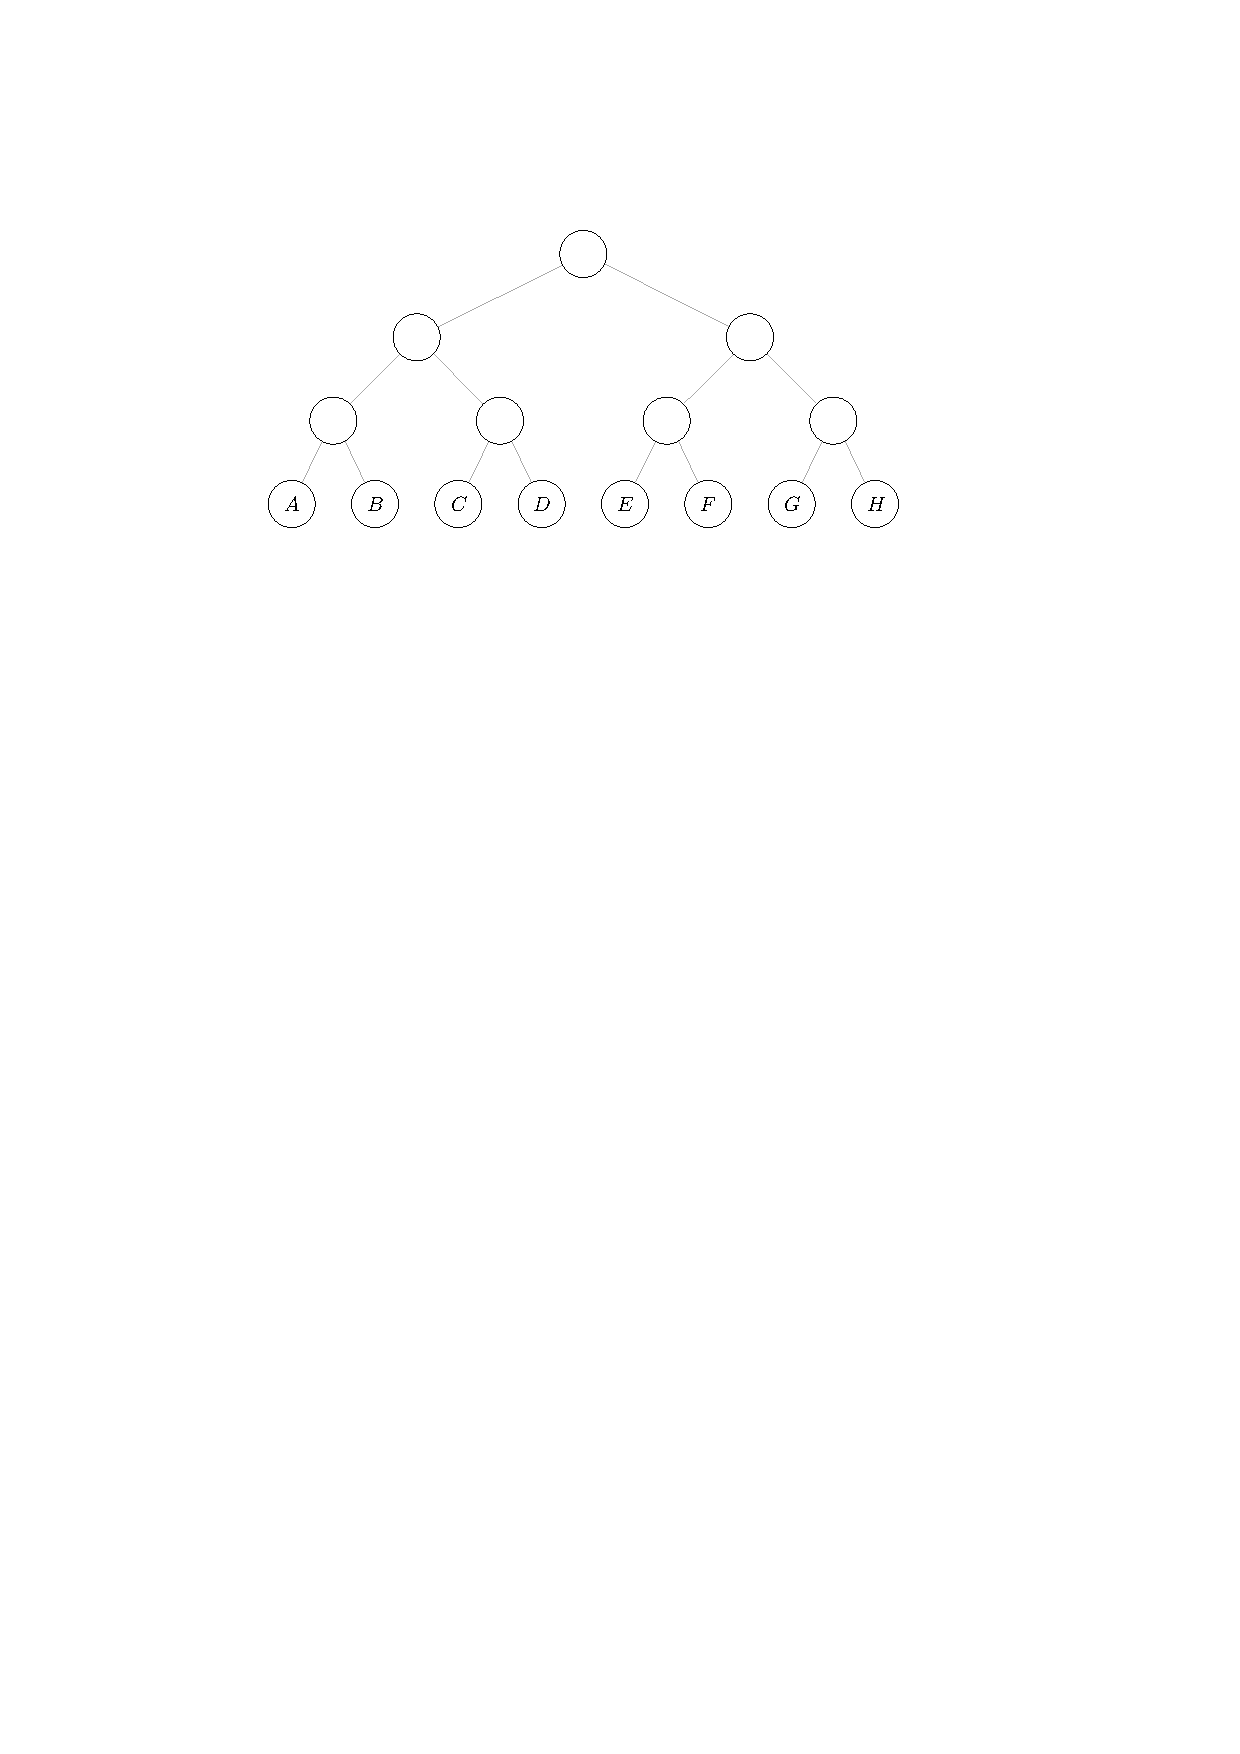
\includegraphics{figures/treekem-tree}
	\end{center}
	\caption{Illustration of a group with users 8 users in the TreeKEM protocol.}\label{fig:treekem-tree}
\end{figure}

The idea behind this tree structure is that it allows for a user creating a commit with a new group key to share the new group key with the group using only a few encryptions, while still updating all the secrets the user knew in the tree in order to recover from a possible compromise (recall that in a PC-CGKA scheme a commit also updates the committer's key material).
To illustrate how a commit is performed and how the new group key is computed, say a user $A$ performs a commit. First we only consider commits without any proposals. TreeKEM specifies two hash functions $\hgen, \hdep \colon \{0, 1\}^{r(\eta)} \to \{0, 1\}^{r(\eta)}$ where $r$ gives the number of bits of randomness used by $\Pi.\gen(1^\eta)$. Let $d = 3$ the depth of user $A$. $A$ will replace all the $d + 1$ nodes on their path to the root (including their leaf) with new nodes $A, p_1, \ldots, p_d$. Although it would be more accurate to say that $A$ just replaces the information stored in the original nodes, and this view makes more sense when implementing the protocol, it will become convenient later to say that $A$ creates new nodes.
The key pairs for the new nodes are sampled as follows. For the leaf node $A$, user $A$ simply samples a key pair by running $\Pi.\gen(1^\eta)$. For the remaining nodes, they first sample $s_1 \from \{0, 1\}^{r(\eta)}$ and compute the key pair of the first parent $p_1$ as $\Pi.\gen(1^\eta, \hgen(s_1))$. For $i \in \{2, \ldots, d\}$ they then compute $s_i \coloneqq \hdep(s_{i - 1})$ and set the key pair of $p_i$ to be $\Pi.\gen(1^\eta, \hgen(s_i))$. The new group key is $k \coloneqq \hdep(s_{d})$.

User $A$ only needs to share (encryptions of) the seeds $s_i$ for the other users to update their view of the tree and compute the new group key:
\begin{itemize}
	\item To share the group key with user $B$, $A$ computes the ciphertext $c_1 \coloneqq \Pi.\enc_{pk_B}(s_1)$. $B$ can then compute the seed $s_1$, then use that to compute the seeds $s_2, \ldots, s_d$, the key pairs of all new nodes on their path to the root and the group key $k$.
	\item To share the new group key with users $C$ and $D$, $A$ computes the ciphertext $c_2 \coloneqq \Pi.\enc_{pk_X}(s_2)$, where $X$ is the parent of the nodes $C$ and $D$. Both $C$ and $D$ know the secret key $sk_X$ of their parent and can decrypt $c_2$.
	\item To share the new group key with users $E, F, G$ and $H$, $A$ computes the ciphertext $c_3 \coloneqq \Pi.\enc_{pk_Y}(s_3)$, where $Y$ is the right child of the root node. Again, all users under $Y$ know $sk_Y$ and can thus decrypt $c_3$.
\end{itemize}
The commit $c$ that $A$ shares with all users includes the ciphertexts $c_1, c_2$ and $c_3$ and the public keys of all new nodes. Figure~\ref{fig:treekem-simple-update} illustrates the commit performed by $A$.

\begin{figure}
	\begin{center}
		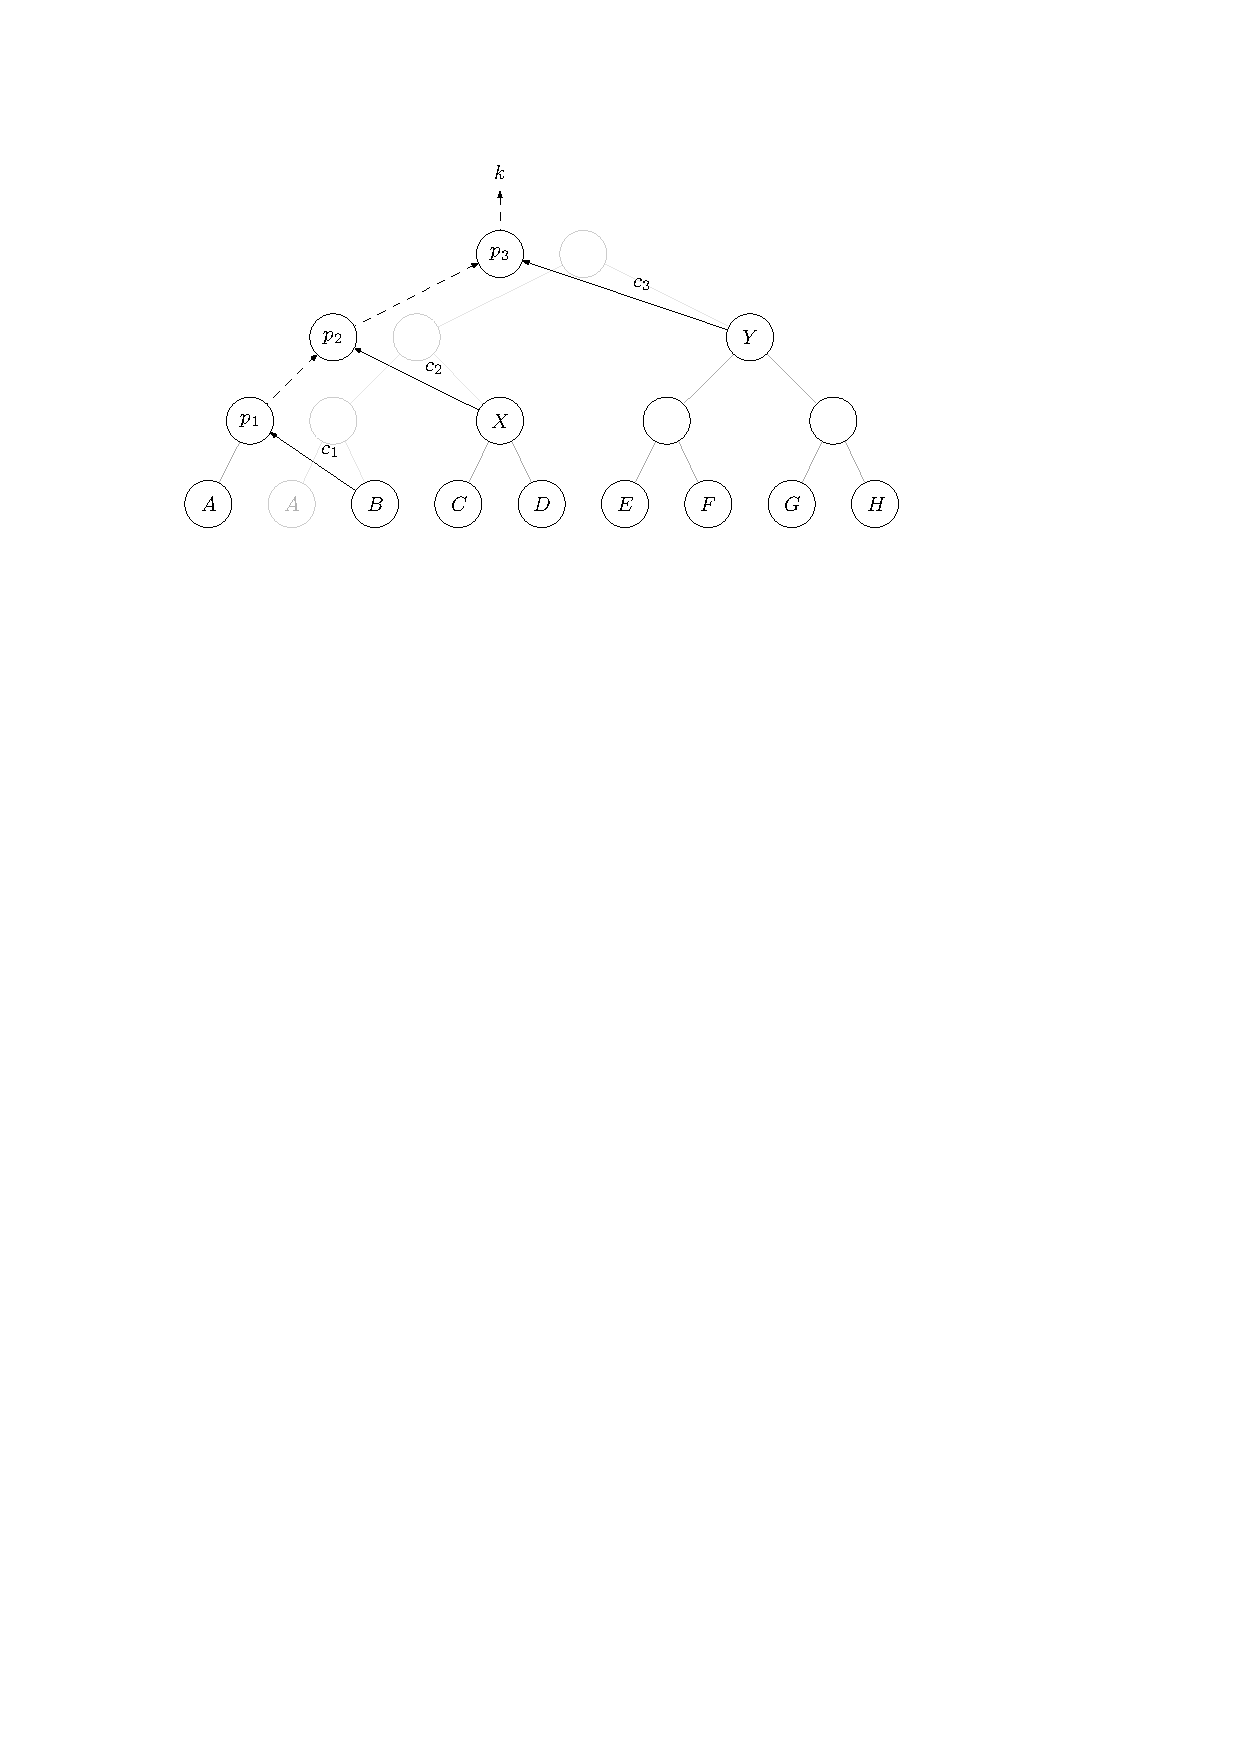
\includegraphics{figures/treekem-simple-update}
	\end{center}
	\caption{The commit by user $A$ described in the text. Dashed directed edges illustrate the fact that the target is related to the source via the hash function $\hdep$. The solid directed edges illustrate the fact that the seed of the target node is encrypted to the public key of the source node.}\label{fig:treekem-simple-update}
\end{figure}

The nodes $B, X$ and $Y$ form the \emph{copath} of $A$: the copath of a node consists of the sibling of each node on the node's path to the root, excluding the root itself. In the ideal case as above, a node performing a commit only has to compute an encryption for each node on it's copath, i.e. logarithmically many in the total number of users.

Things look a bit different if the commit contains a remove proposal. Say user $A$ creates a commit that contains a remove proposal for user $E$. We could just let $A$ replace the nodes on $E$'s direct path $E$ and not encrypt anything for $E$. However, if $A$ were compromised while replacing $E$'s direct path and performed another commit to update their key material after the compromise, the information leaked in the compromise could still be used to compute the new group key, as it includes the secret keys of the nodes on $E$'s direct path.
Instead, all nodes on $E$'s leaf and all nodes on $E$'s direct path are replaced by \emph{blank} nodes: nodes with no associated key pair. Now $A$ would have to encrypt the secret $s_3$ directly to $F$ and to the parent node of $G$ and $H$ in the commit removing user $E$. See Figure~\ref{fig:treekem-remove-user}. A blank leaf node can be populated with a new user. A blank node that is not a leaf will be replaced by a normal node once some user below the node performs a commit. Blank nodes are also useful to represent empty subtrees that have no users.

\begin{figure}
	\begin{center}
		\todo{create figure}
	\end{center}
	\caption{The commit by user $A$ removing user $E$ described in the text.}\label{fig:treekem-remove-user}
\end{figure}

Creating a commit with an update proposal for user $u$ is analogous. The update proposal simply contains the public key of user $u$'s new leaf, while $u$ stored the corresponding secret key locally when creating the proposal. Because we don't want the committer to know the secret keys along $u$'s direct path, we must again blank all these nodes and encrypt to the populated nodes below these blank nodes directly.

Adding a node introduces one more complication. Consider the same group as in Figure~\ref{fig:treekem-tree}, but with the leaf of user $G$ blank. Now say user $A$ would like to add user $G$ to the group.

\todo{Finish explanation of adding a user and unmerged leaves.}

\todo{Define resolution.}

\subsection{Algorithms}

\todo{Describe algorithms.}

% Algorithm $\gen$:
% \begin{itemize}
% 	\item generate init key and private key with $\dhies.\gen$
% 	\item generate leaf node public and private key with $\dhies.\gen$
% 	\item output init key and leaf node public key as public key, and both private keys as secret key
% \end{itemize}
%
% Algorithm $\operatorname{ProposeUpdate}(\sigma)$:
% \begin{itemize}
% 	\item generate $(pk, sk) \dhies.\gen()$
% 	\item output proposal $(pk)$ and store $sk$ in $\sigma$
% \end{itemize}
%
% Algorithm $\operatorname{ProposeAdd}(\sigma, pk_{\mathrm{new}})$:
% \begin{itemize}
% 	\item output proposal $(pk_{\mathrm{new}})$ and store the proposal in $\sigma$
% \end{itemize}
%
% Algorithm $\operatorname{ProposeRemove}(\sigma, v)$:
% \begin{itemize}
% 	\item $v$ is the leaf node of the user to be removed
% 	\item output proposal $(v)$ and store the proposal in $\sigma$
% \end{itemize}

\section{TreeKEM security from SD-GSD security}

\todo{Describe relationship between TreeKEM tree structure and GSD game.}

% To motivate the main result of this section, let us make clear the relation between the PC-CGKA game for TreeKEM and the playing the SD-GSD security game. Consider the tree representing a group in TreeKEM. We can create a matching node in a GSD graph for each node in the tree. Each tree node except the root either has a key pair generated

\todo{Finish statement of Theorem.}

\begin{theorem}
	Let $c, p, u \in \mathbb{N}$. Let $\treekem$ the TreeKEM protocol and recall the hash functions $\hgen, \hdep \colon \{0, 1\}^\lambda \to \{0, 1\}^\lambda$ used in TreeKEM. Let $\dhies$ the DHIES scheme instantiated with a private-key encryption scheme $\Pi_s$. Let $\hdh$ the KDF and $\mathbb{G}$ the group used in $\dhies$. If $\Pi_s$ is $(t, \epsilon)$-EAV secure, the DDH problem is $(t, \epsilon)$-hard in $\mathbb{G}$ and $\hgen, \hdep$ and $\hdh$ are modelled as random oracles, then $\treekem$ is $(\tilde{t}, \tilde{\epsilon}, c, p, u)$-PC-CGKA secure with
	\[
		\tilde{\epsilon} = 2 \cdot (u + 1) \cdot N \cdot \epsilon + \frac{2 \cdot \mdh \cdot N^2}{q} + \frac{\ms \cdot N}{2^{\lambda - 1}},
	\]
	where $N = c \cdot (\lceil \log(u) \rceil + 1) + p$, $\ms$ is an upper bound on the number of queries made to either $\hgen$ or $\hdep$ and $\mdh$ is an upper bound on the number of queries made to $\hdh$, and with
	\[
		\tilde{t} = \ldots
	\]
\end{theorem}

\paragraph{Intuition} \todo{provide outline of the proof and reference proof in \cite{modular-group-messaging}.}


\appendix

\section{Basic cryptographic definitions} \label{sec:preliminaries-appendix}

\subsection{Encryption schemes}

\subsubsection{Private-key encryption}

\begin{definition}[Private-key encryption {\cite[Definition 3.7]{introduction-to-modern-cryptography}}]
	Let $\kappa$ denote the security parameter. A \emph{private-key encryption scheme} $\Pi$ consists of three probabilistic polynomial-time algorithms $(\gen, \enc, \dec)$ such that:
	\begin{enumerate}[1.]
		\item The \emph{key-generation algorithm} $\gen$ takes as input $1^\kappa$ (in unary) and outputs a key $k$. We will write $k \from \gen(1^\kappa)$.
		\item The \emph{encryption algorithm} $\enc$ takes as input a key $k$ and a message $m \in \{0, 1\}^*$, or $m \in \{0, 1\}^{\le l(\kappa)}$ for some function $l$ if the message space is finite, and outputs a ciphertext $c$. We write this as $c \from \enc_k(m)$.
		\item The deterministic \emph{decryption algorithm} $\dec$ takes as input a key $k$ and a ciphertext $c$, and outputs a message $m$ or $\bot$ (denoting an error). We write this as $m = \dec_{k}(c)$.
	\end{enumerate}

	It is required that for every $\kappa$, every key $k$ output by $\gen$, and every message $m$, it holds that $\pr{\dec_k(\enc_k(m)) = m} = 1$ (where the probability is over the randomness of $\enc_k$).
\end{definition}

\subsubsection{Public-key encryption}

In the following definition we will be more explicit about the randomness used by the algorithm $\gen$, as we will require a way to provide the randomness as input.

\begin{definition}[Public-key encryption {\cite[Definition 12.1]{introduction-to-modern-cryptography}}] \label{def:public-key-encryption}
	Let $\eta$ denote the security parameter.
	A \emph{public-key encryption scheme} $\Pi$ consists of three probabilistic polynomial-time algorithms $(\gen, \enc, \dec)$ such that:
	\begin{enumerate}[1.]
		\item The \emph{key-generation algorithm} $\gen$ takes as input $1^\eta$ (in unary) and outputs a pair of keys $(pk, sk)$ (a public and private key). We will write $(pk, sk) \from \gen(1^\eta)$.

		      The public key defines a message space $\mathcal{M}_{pk}$.

		      The algorithm samples $\rho(\eta)$ uniformly random bits to make randomized decisions for some function $\rho$ polynomial in $\eta$. The sequence of random bits $r \in \{0, 1\}^{\rho(\eta)}$ to be used by the algorithm may also be provided as input. We write this as $(pk, sk) = \gen(1^\eta, r)$ to emphasize the fact that the output is deterministic. The distribution over key pairs output by sampling $r \from \{0, 1\}^{\rho(\eta)}$ and running $\gen(1^\eta, r)$ is identical to the distribution over key pairs output by running $\gen(1^\eta)$.


		\item The \emph{encryption algorithm} $\enc$ takes as input a public key $pk$ and a message $m \in \mathcal{M}_{pk}$, and outputs a ciphertext $c$. We write this as $c \from \enc_{pk}(m)$.
		\item The deterministic \emph{decryption algorithm} $\dec$ takes as input a private key $sk$ and a ciphertext $c$, and outputs a message $m$ or $\bot$ (denoting an error). We write this as $m = \dec_{sk}(c)$.
	\end{enumerate}

	It is required that for every $\eta$, every key $(pk, sk)$ output by $\gen$, and every message $m$, it holds that $\pr{\dec_{sk}(\enc_{pk}(m)) = m} = 1$ (where the probability is over the randomness of $\enc_{pk}$).
\end{definition}

\subsection{Security definitions}

\begin{definition}[The IND-CPA game]
	Let $\kappa$ denote the security parameter and let $\Pi$ a private-key encryption scheme. Define the game $\game{\Pi}{\kappa}{IND-CPA}(\adv)$ for an adversary $\adv$:
	\begin{enumerate}[1.]
		\item A key $k \from \gen(1^\kappa)$ is generated.
		\item The adversary $\adv$ is given oracle access to $\Pi.\enc_k$, and outputs a pair of messages $m_0, m_1$ of the same length.
		\item A bit $b \from \{0, 1\}$ is sampled and $\adv$ is given a ciphertext $c \from \enc_k(m_b)$. ($\adv$ continues to have oracle access to $\Pi.\enc_k$.)
		\item $\adv$ outputs a bit $b'$. The output of the game is defined to be $1$ if $b' = b$, and $0$ otherwise.
	\end{enumerate}
\end{definition}

\begin{definition}[IND-CPA security {\cite[Definition 3.21]{introduction-to-modern-cryptography}}]
	For functions $t, \epsilon$ in the security parameter $\kappa$, a private-key encryption scheme $\Pi$ is \emph{$(t, \epsilon)$-IND-CPA-secure} if for all $\kappa$, for any adversary $\adv$ running in time $t(\kappa)$ we have
	\begin{align*}
		\advantage{\Pi}{\kappa}{IND-CPA}(\adv) \coloneqq 2 \cdot \left(\pr{\game{\Pi}{\kappa}{IND-CPA}(\adv) = 1} - \frac{1}{2}\right) \le \epsilon(\kappa).
	\end{align*}
\end{definition}

We will make use of a weaker form of security called ``indistinguishability in the presence of an eavesdropper'' \cite{introduction-to-modern-cryptography} and will refer to it as ``EAV security''. It is identical to IND-CPA security with the sole exception that the adversary does not have access to an encryption oracle.

\begin{definition}[The EAV game]
	Let $\kappa$ denote the security parameter and let $\Pi$ a private-key encryption scheme. Define the game $\game{\Pi}{\kappa}{EAV}(\adv)$ for an adversary $\adv$:
	\begin{enumerate}[1.]
		\item A key $k \from \gen(1^\kappa)$ is generated.
		\item The adversary $\adv$ outputs a pair of messages $m_0, m_1$ of the same length.
		\item A bit $b \from \{0, 1\}$ is sampled and $\adv$ is given a ciphertext $c \from \enc_k(m_b)$.
		\item $\adv$ outputs a bit $b'$. The output of the game is defined to be $1$ if $b' = b$, and $0$ otherwise.
	\end{enumerate}
\end{definition}

\begin{definition}[EAV security {\cite[Definition 3.8]{introduction-to-modern-cryptography}}]
	A private-key encryption scheme $\Pi$ is \emph{$(t, \epsilon)$-EAV-secure} if for all $\kappa$, for any adversary $\adv$ running in time $t(\kappa)$ we have
	\begin{align*}
		\advantage{\Pi}{\kappa}{EAV}(\adv) \coloneqq 2 \cdot \left(\pr{\game{\Pi}{\kappa}{EAV}(\adv) = 1} - \frac{1}{2}\right) \le \epsilon(\kappa).
	\end{align*}
\end{definition}


\begin{lemma}
	Let $\Pi$ a private-key encryption scheme. If $\Pi$ is $(t, \epsilon)$-IND-CPA-secure, then $\Pi$ is $(t, \epsilon)$-EAV-secure.
\end{lemma}
\begin{proof}
	This follows immediately from the fact that any EAV adversary is also an IND-CPA adversary.
\end{proof}

When analyzing the advantage of an adversary we may make use of the following well known equality.

\begin{lemma}
	Let $X$ a Bernoulli random variable and $b \from \{0, 1\}$ (where $X$ and $b$ are not necessarily independent). Then for $x \in \{0, 1\}$
	\[
		2 \cdot \left(\pr{X = b} - \frac{1}{2}\right) = \pr{X = x \mid b = x} - \pr{X = x \mid b = 1 - x}.
	\]
	In particular, if $\adv$ is an adversary with output in $\{0, 1\}$ playing a game where a bit $b \from \{0, 1\}$ is sampled, then for $x \in \{0, 1\}$
	\begin{equation} \label{eq:advantage-equality}
		2 \cdot \left(\pr{b \from \adv} - \frac{1}{2}\right) = \pr{x \from \adv \mid b = x} - \pr{x \from \adv \mid b = 1 - x}.
	\end{equation}
\end{lemma}
\begin{proof}
	Let $x \in \{0, 1\}$. We have
	\begin{align*}
		2 \cdot \left(\pr{X = b} - \frac{1}{2}\right) & = 2 \cdot \left(\pr{X = x \mid b = x} \cdot \frac{1}{2} + \pr{X = 1 - x \mid b = 1 - x} \cdot \frac{1}{2} - \frac{1}{2}\right) \\
		                                              & = \pr{X = x \mid b = x} + \pr{X = 1 - x \mid b = 1 - x} - 1                                                                    \\
		                                              & = \pr{X = x \mid b = x} - (1 - \pr{X = 1 - x \mid b = 1 - x})                                                                  \\
		                                              & = \pr{X = x \mid b = x} - \pr{X = x \mid b = 1 - x}.
	\end{align*}
\end{proof}

\subsection{The Decisional Diffie-Hellman problem}

\begin{definition}[Group-generation algorithm {\cite[Section 9.3.2]{introduction-to-modern-cryptography}}]
	A \emph{group-generation algorithm} $\mathcal{G}$ is a probabilistic polynomial-time algorithm that takes as input $1^\eta$ and outputs $(\mathbb{G}, q, g)$, where $\mathbb{G}$ is (a description of) a cyclic group with order $q$ and $g \in \mathbb{G}$ is a generator. A group element is represented as a bit-string of length at most $\gamma(\eta)$. We write $(\mathbb{G}, q, g) \from \mathcal{G}(1^\eta)$.
\end{definition}

\begin{definition}[The Decisional Diffie-Hellman (DDH) problem {\cite[Section 9.3.2]{introduction-to-modern-cryptography}}]
	Let $\mathcal{G}$ a group-generation algorithm.
	Define the game $\game{\mathcal{G}}{\eta}{DDH}(\adv)$ for an adversary $\adv$:
	\begin{enumerate}[1.]
		\item $\mathcal{G}(1^\eta)$ is run to obtain $(\mathbb{G}, q, g)$, and exponents $x, y \from [q]$ and a bit $b \from \{0, 1\}$ are sampled.
		\item The adversary $\adv$ is given $\mathbb{G}$, $q$, $g$, $h_1 \coloneqq g^x, h_2 \coloneqq g^y$ and
		      \[
			      k = \begin{cases}
				      g^{x \cdot y} & b = 0 \\
				      \tilde{k}     & b = 1
			      \end{cases}
		      \]
		      where $\tilde{k} \from \mathbb{G}$.
		\item $\adv$ outputs a bit $b'$. The output of the game is defined to be $1$ if $b' = b$, and $0$ otherwise.
	\end{enumerate}
\end{definition}

\begin{definition}[Hardness of the DDH problem {\cite[Definition 9.64]{introduction-to-modern-cryptography}}]
	The DDH problem is \emph{$(t, \epsilon)$-hard relative to} $\mathcal{G}$ if for all $\eta$, for any adversary $\adv$ running in time $t(\eta)$ we have
	\begin{align*}
		\advantage{\mathcal{G}}{\eta}{DDH}(\adv) \coloneqq 2 \cdot \left(\pr{\game{\mathcal{G}}{\eta}{DDH}(\adv) = 1} - \frac{1}{2}\right) \le \epsilon(\eta).
	\end{align*}
\end{definition}

\subsection{The Random Oracle Model} \label{sec:rom}

We will work in the commonly used Random Oracle Model (ROM) to prove our results. We refer the reader to \cite[Chapter 6.5]{introduction-to-modern-cryptography} for an informal overview of the ROM and to \cite{rom} for the original work that introduced the model. The ROM introduces the concept of a \emph{random oracle}. If a function $H : A \to B$ is modelled as a random oracle, then certain assumptions are made about what an adversary $\adv$ knows about $H$ and how it interacts with it:
\begin{itemize}
	\item From $\adv$'s perspective, $H$ is a black-box function. The only way for $\adv$ to interact with $H$ is for it to provide a value $a \in A$ and get back $H(a)$, and this is the only way for $\adv$ to learn $H(a)$. We say that $\adv$ \emph{queries} $H(a)$ or that $\adv$ \emph{queries $H$ for $a$}. This well-defined interface of $\adv$ to $H$ implies that a reduction can extract the queries that $\adv$ makes to $H$.
	\item From $\adv$'s perspective, $H$ is a random variable, sampled u.a.r.\ from the set of all functions from $A$ to $B$. Thus, if $\adv$ queries $H$ for some $a \in A$ that it has not queried before, the value $H(a)$ is a random variable uniformly distributed in $B$ from $\adv$'s perspective.
\end{itemize}
We do not rely on the property known as ``programmability'' in this work.


\section{Appendix}

\subsection{Proof of Lemma~\ref{lemma:mis-eav-from-eav}} \label{sec:mis-eav-from-eav-proof}

\begin{proof}[of Lemma~\ref{lemma:mis-eav-from-eav}] Note that since the message space is finite, the time to encrypt a message is bounded. As outlined before Lemma~\ref{lemma:mis-eav-from-eav}, the lemma follows from a simple hybrid argument. Let $q$ a function in $\kappa$, let $\kappa$ arbitrary and let $\adv$ an arbitrary MIS-EAV adversary running in time $\tilde{t}(\kappa)$ and making at most $q(\kappa)$ queries. Define the sequence of hybrid games $H_0, \ldots, H_q$ where in the game $H_i$ the first $i$ encryptions given to the adversary encrypt $m_1$ and all remaining encryptions encrypt $m_0$. We will write
	\[
		\pr{0 \from \adv \mid H_i}
	\]
	for the probability of $\adv$ outputting $0$ when playing the hybrid game $H_i$.

	Let $i \in [q]$. Construct an EAV adversary $\adv'$ that behaves as follows:
	\begin{enumerate}[1.]
		\item $\adv'$ runs $\adv$ and gets $q, m_0, m_1$.
		\item $\adv'$ outputs the messages $m_0, m_1$ and gets a ciphertext $c$ from the challenger.
		\item $\adv'$ gives the ciphertexts $c_1, \ldots, c_q$ to $\adv$ where
		      \[
			      c_j = \begin{cases}
				      \Pi.\enc_{k_j}(m_1) & i < j \\
				      c                   & i = j \\
				      \Pi.\enc_{k_j}(m_0) & i > j
			      \end{cases}
		      \]
		      and $k_j \from \Pi.\gen(1^\kappa) \; \forall j$.
		\item $\adv'$ outputs whatever bit $\adv$ outputs.
	\end{enumerate}
	Now consider the value of the bit $b$ sampled in $\game{\Pi}{\kappa}{EAV}(\adv')$. If $b = 0$, then the first $i - 1$ ciphertexts that $\adv$ received were encryptions of $m_1$ and the remaining ciphertexts were encryptions of $m_0$, where all encryptions were under keys sampled independently with $\Pi.\gen$. Thus, from the view of $\adv$ everything followed the same distribution as in the game $H_{i - 1}$ and
	\[
		\pr{0 \from \adv' \mid b = 0} = \pr{0 \from \adv \mid H_{i - 1}}.
	\]
	Analogously, in the case $b = 1$ the first $i$ ciphertexts received by $\adv$ were encryptions of $m_1$ and the rest encryptions of $m_0$, so
	\[
		\pr{0 \from \adv' \mid b = 1} = \pr{0 \from \adv \mid H_{i}}.
	\]
	Then
	\begin{align} \label{eq:eav-to-mis-eav-hybrid-distinguisher}
		\begin{split}
			\begin{split}
				\pr{0 \from \adv \mid H_{i - 1}} - & \pr{0 \from \adv \mid H_{i}} \\
				& = \pr{0 \from \adv' \mid b = 0} - \pr{0 \from \adv' \mid b = 1}
			\end{split} \\
			& \stackrel{\mathclap{\eqref{eq:advantage-equality}}}{=} \advantage{\Pi}{\kappa}{EAV}(\adv')                                         \\
			& \le \epsilon
		\end{split}
	\end{align}
	by $(t, \epsilon)$-EAV security of $\Pi$ since $\adv'$ runs in time $\tilde{t} + \mathcal{O}(q \cdot (t_{\gen} + t_{\enc})) = t$.

	Now let $b$ be the bit sampled in the MIS-EAV game. Notice that
	\[
		\pr{0 \from \adv \mid b = 0} = \pr{0 \from \adv \mid H_0}
	\]
	and
	\[
		\pr{0 \from \adv \mid b = 1} = \pr{0 \from \adv \mid H_q}.
	\]
	Then
	\begin{align*}
		\advantage{\Pi}{\kappa}{MIS-EAV}(\adv) & \stackrel{\mathclap{\eqref{eq:advantage-equality}}}{=} \; \pr{0 \from \adv \mid b = 0} - \pr{0 \from \adv \mid b = 1} \\
		                                       & = \pr{0 \from \adv \mid H_0} - \pr{0 \from \adv \mid H_q}                                                             \\
		                                       & = \sum_{i = 1}^{q} \pr{0 \from \adv \mid H_{i - 1}} - \pr{0 \from \adv \mid H_i}                                      \\
		                                       & \stackrel{\mathclap{\eqref{eq:eav-to-mis-eav-hybrid-distinguisher}}}{\le} q \cdot \epsilon.
	\end{align*}
\end{proof}


\backmatter

\bibliographystyle{plain}
\bibliography{refs}

% 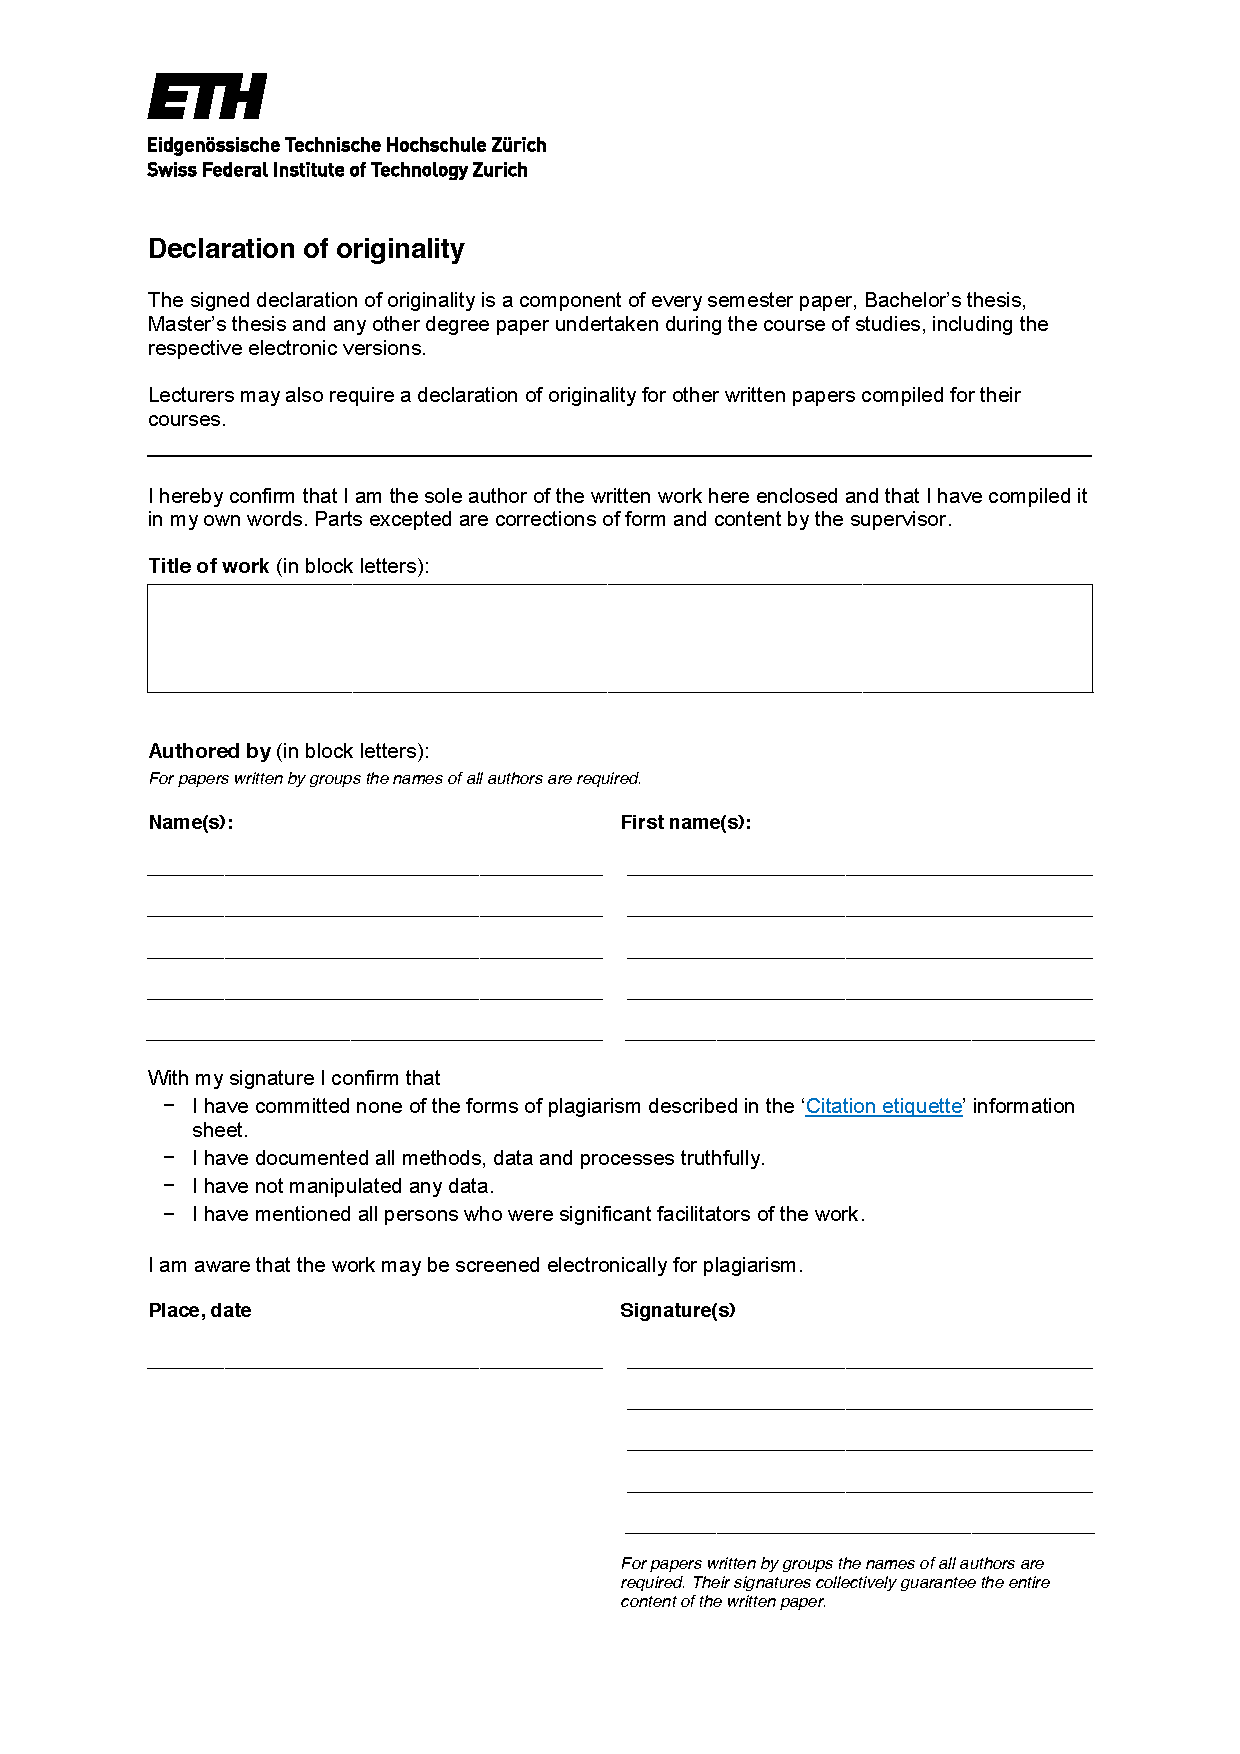
\includepdf[pages={-}]{declaration-originality.pdf}

\end{document}
